%
% Header die benutzt werden sollen
%
\documentclass[
  pdftex,
  fontsize=12pt,          % Schriftgroesse
  DIV10,                  % Angabe bzgl Bestimmung der Seitenabstaende
  ngerman,                % fuer Umlaute, Silbentrennung etc.
  paper=a4,               % Papierformat
  twoside=false,          % einseitiges Dokument
  titlepage,              % es wird eine Titelseite verwendet
  parskip=half,           % Abstand zwischen Absaetzen (halbe Zeile)
  headings=normal,        % Groesse der Ueberschriften verkleinern
  listof=nochaptergap,    % Verzeichnisse im Inhaltsverzeichnis auffuehren.
  bibliography=totoc,     % Literaturverzeichnis im Inhaltsverzeichnis auffuehren
  index=totoc,            % Index im Inhaltsverzeichnis auffuehren
  captions=tableheading,  % Beschriftung von Tabellen oberhalb ausgeben
  bookmarksopen,
  bookmarksnumbered,
  final                   % Status des Dokuments (final/draft)
]{scrreprt} 

\usepackage[T1]{fontenc}
\usepackage[utf8]{inputenc}
\usepackage[ngerman]{babel}
\usepackage{palatino}

% Zeilenabstand
\usepackage[onehalfspacing]{setspace}

% Code
\usepackage{listings}
\lstdefinestyle{sharpc}{float,
	language=[sharp]C, 
	frame=single,  
	keywordstyle=\bfseries\color{green!40!black},
	commentstyle=\itshape\color{purple!40!black},
	identifierstyle=\color{blue},
	stringstyle=\color{orange}, 
	showstringspaces=false, 
	showspaces=false, 
	numbers=left, 
	captionpos=b, 
	belowcaptionskip=4pt,
	basicstyle=\ttfamily}

%Tabellen
\usepackage{array}
\usepackage{tabularx}
\usepackage{supertabular}
\usepackage{longtable}

%Grafiken
\usepackage[pdftex]{graphicx}
\usepackage{wrapfig}
\usepackage[svgnames]{xcolor}
\usepackage{float}
\usepackage{pdfpages}

%Sprache und Anführungszeichen
\usepackage[babel,german=quotes]{csquotes}
\usepackage{eurosym}

%Abstände
\usepackage[left=2.5cm, right=2.5cm, top=2.5cm, bottom=2.5cm ]{geometry}

% Pakete um Textteile drehen zu können, oder eine Seite Querformat anzeigen kann.
\usepackage{rotating}
\usepackage{lscape}

%Literaturverweise
\usepackage[style=numeric, backend=biber, citestyle=numeric, dashed=false]{biblatex}

% Hurenkinder und Schusterjungen verhindern
% http://projekte.dante.de/DanteFAQ/Silbentrennung
\clubpenalty=10000
\widowpenalty=10000
\displaywidowpenalty=10000

%Abkürzungsverzeichnis
\usepackage[printonlyused]{acronym}

% Fussnoten
\usepackage[hang, multiple, stable]{footmisc}

\usepackage[%
%	pdftitle={\pdftitel},
%	pdfauthor={\autor},
%	pdfsubject={\arbeit},
%	pdfcreator={pdflatex, LaTeX with KOMA-Script},
%	pdfpagemode=UseOutlines, % Beim Oeffnen Inhaltsverzeichnis anzeigen
%	pdfdisplaydoctitle=true, % Dokumenttitel statt Dateiname anzeigen.
%	pdflang=de % Sprache des Dokuments.
]{hyperref}
\usepackage[all]{hypcap}


% Nummerierung ohne Kapitel-Nr.
\usepackage{chngcntr}
\counterwithout{figure}{chapter}
\counterwithout{equation}{chapter}
\counterwithout{footnote}{chapter}
\counterwithout{table}{chapter}
%
% EOF
%
\addbibresource{lib.bib}
\renewcommand{\bibname}{Literaturverzeichnis} 

\setlength{\parindent}{0mm}

\begin{document}
%Deckblatt
%
% Deckblatt
%

\begin{titlepage}

	\begin{center}
		% Logos der Firma und DHBW
		\vspace*{0cm}
		%\includegraphics[width=8cm]{images/firma}
		\hfill
		%\includegraphics[width=6cm]{images/dhbw-logo}\\ [3cm]
		%Titel, Typ der Arbeit, Studiengang
		{\Large \textbf{Titel} } 	\\ [2cm]
		{\Large  \scshape \textbf{Studienarbeit}}	\\ [2cm]
		{\large des Studiengangs Angewandte Informatik}	\\ [0.5cm]
		{\large an der Dualen Hochschule Baden-Württemberg Karlsruhe}	\\[0.5cm]
		
		
		{\large von} 	\\ [0.5cm]
		%Autor und Abgabedatum
		{\large \bfseries \textbf{Mehmet Ali Incekara \& Tom Wolske}}	\\ [1cm]
		{\large Abgabedatum \today}
		\vfill
	\end{center}
	
	\begin{tabular}{l@{\hspace{2cm}}l}
	\textbf{Bearbeitungszeitraum}			&	12 Wochen		\\
	\textbf{Matrikelnummer}					&	12345678 \& 1156973		\\
	\textbf{Kurs}							&	TINF14B2			\\
	\textbf{Gutachter der Studienakademie}	&	Prof. Dr. Kay Berkling	\\
	\end{tabular}

\end{titlepage}

%
% EOF
%

\renewcommand{\thepage}{\Roman{page}}
\setcounter{page}{1}
% Formale Erklärungen
%\thispagestyle{empty}

\section*{Erklärung}
% Seite 8
% http://studium.ba-bw.de/fileadmin/media/allgemein/bestimmungen/btechnik/richtlinien/Richtlinien_Praxismodule_Studien_und_Bachelorarbeiten_2011.pdf
\vspace*{2em}

Gemäß \S 5 (2) der \enquote{Studien- und Prüfungsordnung DHBW Technik} vom 18. Mai 2009 erkläre ich hiermit,
\begin{enumerate}
\item dass ich die vorliegende Arbeit selbstständig verfasst und keine anderen als die
angegebenen Quellen und Hilfsmittel verwendet habe. 
\item dass die Übernahme von Zitaten und Gedankengut anderer Autoren gekennzeichnet wurde.
\item dass die eingereichte elektronische Fassung exakt mit der schriftlichen übereinstimmt.
\item dass ich die Projektarbeit keiner externen Prüfung vorgelegt habe.
\end{enumerate}

\vspace{3em}

\begin{tabular}{lp{2em}l}
 Karlsruhe, den \today  && \hspace{7cm} \\\cline{1-1}\cline{3-3}
 Ort, Datum     &&  Tom Wolske
\end{tabular} 

\begin{tabular}{lp{2em}l}
 Karlsruhe, den \today  && \hspace{7cm} \\\cline{1-1}\cline{3-3}
 Ort, Datum     &&  Mehmet Ali Incekara
\end{tabular} 

%Abstract
%\thispagestyle{empty}

\section*{Abstract}

\pagebreak

\section*{Zusammenfassung}

% Inhaltsverzeichnis

\tableofcontents
\newpage
\newpage

\phantomsection
\addcontentsline{toc}{chapter}{Abkürzungsverzeichnis}
\chapter*{Abkürzungsverzeichnis}
\begin{acronym}[SDK]

\acro{SDK}{Software Development Kit}

\end{acronym}
\newpage
\listoffigures
%\listoftables
\newpage
\counterwithout{lstlisting}{chapter}
\lstlistoflistings

%--> Speichern der Zahl fürs umsetzten zurück auf römische 
\newcounter{SeitenzahlSpeicher}
\setcounter{SeitenzahlSpeicher}{\value{page}}


\newpage

%Arabische Nummerierung
\renewcommand{\thepage}{\arabic{page}}
\setcounter{page}{1}

%Kapitel
\chapter{Einleitung}

Spiele, jeder kennt sie und spielt regelmäßig welche. Sie sind ein fester Bestandteil unserer Kultur und das schon seit tausenden Jahren. Die ersten Gesellschaftsspiele wurden noch im Sand mit Stöcken oder Steinen gespielt. Eines der frühesten Spiele wird auch heutzutage noch gespielt, dabei handelt es sich um Mühle, ein Spiel welches die Ägypter vor bereits 3000 Jahren gespielt haben.\footnote{vgl. gesellschaftsspiele.de \cite{spiele} (2015)} Spiele haben sich seit dem jedoch weiterentwickelt und dienen heutzutage nicht nur zum munteren Zeitvertreib. 

Ob als Brett, Karten oder Glücksspiel, Spiele sind überall zu finden und jeder kann sie spielen. Seit 1972 entwickeln sich darüber hinaus weitere Spiele, Videospiele. Sie nutzen die immer größer werdende Rechenleistung von Computern aus, um uns immer realistisch aussehender Spiele zu liefern. 
Um den Überblick über die Vielzahl an Videospielen zu behalten, haben sich in den letzten Jahren verschiedene Plattformen etabliert, die versuchen dem Nutzer das zu bieten, was sie suchen. Dabei stellen diese viele verschiedene Arten von Spielen für die Gamer bereit, die einen beim Spielen die Zeit vergessen lassen. Beispiele für solche Plattformen sind unter anderem Steam, Uplay oder Origin.

Allerdings können Spiele uns nicht nur die Zeit vergessen lassen und für heitere Stunden sorgen, sie können uns auch Wissen vermitteln. Sei es beispielsweise durch eine Geschichte die sich real abgespielt hat, wie der erste Weltkrieg. Dieses Wissen wird unterbewusst an den Nutzer vermittelt, ohne das er aktiv versucht dieses zu lernen.

Für diesen Zweig hat sich eine eigene Branche entwickelt, welche sich mit Lernspielen befasst und versucht uns, über Videospiele, neues Wissen zu vermitteln. Viele dieser Spiele nutzen bekannte Figuren, welche die Kinder aus dem Fernsehen kennen, um dieses Wissen zu vermitteln.

Diese Spiele werden hauptsächlich in den Schulen eingesetzt, um den Kindern wissen spielerisch zu vermitteln. Jedoch profitiert nicht jedes Kind von diesem Vorteil. Sei es, weil die Schule keine Computer hat oder weil das Kind nicht eine Schule besuchen kann. Für diesen Zweck wurde die Plattform Hone\footnote{siehe \url{http://hone-kids.herokuapp.com/}} entwickelt, mit der Kinder, die nicht zur Schule gehen können, die Möglichkeit haben, Wissen zu erlangen. 

\section{Motivation}
Bei Hone handelt es sich um eine Spielplattform auf der sich Kinder, bevorzugt aus Regionen in denen Bildung mangelhaft ist, anmelden können. Auf dieser Web-Plattform gibt es für Kinder die Möglichkeit neue Lernspiele für verschiedene Plattformen herunterzuladen. Zusätzlich gibt es eine Ansicht der gelernten Kompetenzen. 

Dieses Konzept hat zwei wesentliche Nachteile für die Benutzer. Für die Verwendung der Web-Plattform wird ein Computer benötigt und gerade weil Spiele für verschiedene Plattformen angeboten werden können, benötigt das Kind mehrere Geräte. Neben diesen Nachteilen, ist das Aussehen und die Bedienung dieser Plattform nicht reizvoll für Kinder gestaltet.

Mehr Kinder als je zuvor in der Geschichte arbeiten täglich mit immer neueren und besseren technischen mobilen Geräten. Deshalb soll eine mobile Applikation, kurz App, für Smartphones entwickelt werden, in der die Kinder auf spielerischer weise Fortschritte machen. Durch die Umsetzung als App wird den Kindern eine Plattform angeboten, mit welcher sie unabhängig und jederzeit auf die Lerninhalte zugreifen können. Ein weiterer Vorteil ist, dass die Kinder den technischen Umgang mit Smartphones lernen. Die App wird unabhängig von Hone funktionieren und es werden keine Inhalte und Funktionen übernommen.

\section{Ziel der Arbeit}

Das Ziel dieses Projektes ist es den Kindern eine Möglichkeit zu geben, mit der sie jederzeit, überall und einfach auf die Lerninhalte zugreifen und spielerisch neues Wissen erwerben können.

Dabei ist es nicht das Ziel die Lerninhalte direkt in der App abzufragen sondern Lernspiele für Smartphones anzubieten, welche es in korrekter Reihenfolge freizuschalten und zu spielen gilt.

Das Ziel dieser Arbeit ist die Vorgehensweise, Bedingungen, Probleme zu dokumentieren. Mit dieser Dokumentation soll gewährleistet werden, dass dieses Projekt von allen Verstanden wird.

\section{Aufbau der Arbeit}

Die einzelnen Kapitel dieser Arbeit repräsentieren die notwendigen Schritte, das Ziel dieses Projektes zu erreichen.

Bevor überhaupt Anforderungen spezifiziert werden können, müssen zunächst die Ideen und Gründe hinter diesem Projekt beschrieben werden. Das nächste Kapitel behandelt deshalb das Konzept der App. Zudem wird das beschriebene Konzept von anderen Spielkonzepten abgegrenzt, um die Unterschiede klarzustellen.

Im darauf folgendem dritten Kapitel wird das zum Projekt dazugehörende Software Requirements Specifikation behandelt. Dies dient zur Spezifikation der App. Neben funktionalen Anforderungen werden hier auch nicht-funktionale Anforderungen festgeschrieben.

Anschließend wird auf die technischen Grundlagen für die Umsetzung eingegangen. Dabei wird die gewählte Entwicklungsumgebung und weitere notwendigen Technologien beschrieben.

Darauf aufbauend wird im fünften Kapitel die Umsetzung behandelt. Dabei wird auf Besonderheiten und Probleme in der Entwicklungsphase eingegangen. Dafür werden die einzelnen Komponenten der App beschrieben.

Abgeschlossen wird diese Arbeit mit einem Fazit und Ausblick, in dem der weitere Werdegang des Projektes geschildert wird.
\chapter{NoRPG}

%%%%DAS WAR MEINE BESCHREIBUNG IM SRS VIELLEICHT WILLST DU WAS ÜBERNEHMEN WIE DIE QUELLE OR STH ENJOY

%Bei NoRPG handelt es sich um eine Gamifizierung einer Lernspielplattform für Android. NoRPG stellt unterschiedlichste Lernspiele bereit und ist dabei wie ein Rollenspiel aufgebaut und besitzt auch dieselben charakteristischen Eigenschaften eines Rollenspiels. Eine charakteristische Eigenschaft von Rollenspielen ist, dass der Spielende in die Rolle realer Menschen, fiktiver Figuren, Tiere oder auch Gegenstände übernimmt\footnote{vgl. Warwitz & Rudolf \cite{rpgSinn} Seite 78ff.}. 
		
%Jedoch handelt es sich bei NoRPG letztendlich nicht um ein klassisches Rollenspiel sondern immer noch um eine Lernspielplattform und bietet Lernspiele zum Herunterladen an. NoRPG soll durch die Eigenschaften eines Rollenspiels die Spieler dazu anregen, weitere Lernspiele herunterzuladen und zu spielen. Dabei wird die Software die Lernspiele in einer festgelegten Reihenfolge anbieten und mit Hilfe einer Anzeige, den aktuellen Fortschritt des Spielers festhalten.	
		%%%%%%%%%%%%%%%%%%%%%%%%%%%%%%%%%%%%%%%%%%%%%%%%%%%%%%%%%%%%%%%%%%%%%%%%%
		
%Bei NoRPG handelt es sich um eine Gamifizierung einer Lernspielplattform für Android.  <-- Vielleicht nmoch ein allgemeiner satz davor bevor du in das geschehen reingehst :D
Bei NoRPG handelt es sich um ein Spiel, welches an ein Role Player Game (RPG) erinnern soll. Bei RPGs spielt der Spieler einen Charakter in einer fiktiven Welt. Dabei gibt es eine Story die während des Spielens erlebt wird. Damit diese Geschichte voran geht, muss der Spieler verschiedene Missionen bzw. Quests erledigen, um einen Fortschritt im Spiel zu erlangen. Dabei handelt es sich um die verschiedensten Aufgaben. Darüber hinaus sammelt der Spieler Objekte in der Welt, welche er anschließend im Spiel nutzen kann. Ein Beispiel für solche Spiele ist das Spiel The Witcher 3, welches auf diesen Prinzipien aufbaut. %todo: <-- verlinkung auf wichter 3 like: "für weitere Informationen:..."
	
Darüber hinaus gibt es noch sogenannte MMORPGs, Massive Multiplayer Online Role Player Game. Dabei gibt es wie bei RPGs eine Story und Quests, allerdings kann man auch auf andere Spieler treffen und mit diesen gemeinsam spielen. Das wohl berühmteste MMORPG ist dabei World of Warcraft %todo: auch hier ein link für weitere Informationen
vom Entwickler Blizzard. Hier kann der Spieler zwischen verschiedenen Klassen einen Charakter auswählen, von menschenähnlichen bis zu skurrilen Gestalten. Jede dieser Klassen hat verschiedene Fähigkeiten, welche sich auf den Spielverlauf auswirken. Darüber hinaus gibt es in MMORPGs verschiedene Events, an denen die Spieler gemeinsam versuchen eine Quest zu erfüllen. Dieser Multiplayermodus grenzt die MMORPGs von den RPG ab.

NoRPG hat keine Multiplayer Möglichkeiten und wird deswegen nur als ein RPG klassifiziert. Allerdings muss der Spieler keine Quests erfüllen, wie sie aus anderen Spielen bekannt sind. Der Nutzer muss andere Spiele spielen, damit der Spieler voran schreiten kann. Deshalb wurde sich für den Namen NoRPG entschieden, da es sich bei dem Spiel um ein RPG handelt, aber nicht alle klassischen Eigenschaften eines RPGs besitzt.
	
NoRPG ist ein Spiel, welches versucht Bildung für jeden erreichbar zu machen. Dieses Ziel ist dabei in den Global Goals definiert. Dabei handelt es sich um 17 Ziele welche bis 2030 Umgesetzt werden sollen, um das Leben für alle Menschen auf der Welt zu verbessern\footnote{vgl. Global Goals \cite{global} (2017)}. 2015 haben 193 Weltführer diese Unterzeichnet und begonnen dieses umzusetzen. Dabei sind diese Ziele umfangreich und reichen von einem besseren Umgang mit den uns zur Verfügung stehenden Ressourcen bis hin zu qualitativ hochwertiger Bildung für jeden und kostenlos.

NoRPG unterstützt dabei das Ziel hochwertige Bildung für jeden Zugänglich zu machen, da die App für jeden frei, kostenlos und überall angeboten wird. Dieses Ziel hat weitere Unterziele, wobei nun kurz auf die für NoRPG relevanten Unterziele eingegangen wird.

\begin{itemize}
\item Bis 2030 sicherstellen, dass alle Mädchen und Jungen gleichberechtigt eine kostenlose und hochwertige Grund- und Sekundarschulbildung abschließen, die zu brauchbaren und effektiven Lernergebnissen führt.

Dieses Unterziel wird in NoRPG dahingegen unterstützt, dass die Common Core State Standards implementiert werden. Dies sind Standards für Unterrichtsfächer und beschreiben den zu lernenden Inhalt für Kinder in den verschiedenen Klassen. Da NoRPG für alle kostenfrei zugänglich ist und Mädchen und Jungen gleichberechtigt sind, werden auch diese zwei Aspekte des Unterziels unterstützt. Die Standards werden dabei von den zu Verfügung gestellten Spielen erfüllt.

\item Aufbau und Weiterentwicklung von Bildungseinrichtungen, die kinder- und behindertengerecht und geschlechtsspezifisch sind und für alle eine sichere, gewaltfreie, integrative und effektive Lernumgebung bieten. %todo: vielleciht 2 sätze :P

Da NoRPG keine Bildungseinrichtung ist wird dieses Unterziel nur bedingt erfüllt. NoRPG bietet Kindern jedoch eine sichere, gewaltfreie, integrative und effektive Lernumgebung, wodurch dieses Ziel allerdings zum Teil erfüllt wird. Darüber hinaus ist diese Umgebung für Kinder ausgelegt. Geschlechtsspezifisch ist das Spiel nur dahingehend, dass die Kinder zu Beginn das Geschlecht ihres Charakters auswählen.

\end{itemize}


	
\section{Gedanken} %todo: anderer Kapitelname: weil es handelt nur von Gamifikation

Dieses Ziel der Global Goals wird dabei durch Gamification umgesetzt. Bei Gamification oder Gamifizierung handelt es sich um das nutzen von spielespezifischen Eigenschaften, welche außerhalb von Spielen angewendet werden. Ein Beispiel dafür ist PayBack. Dabei sammeln die Nutzer bei jedem Einkauf Punkte. Diese Punkte können die Kunden dann gegen Prämien eintauschen. In Videospielen sammeln die Spieler zum Beispiel Münzen um diese anschließend einzutauschen. 

Gamification setzt darüber hinaus auch weitere erfolgreiche Prinzipien aus Videospielen um, damit die Nutzer Spaß daran haben, das Produkt zu nutzen. Dadurch soll die Motivation gesteigert werden, NoRPG zu verwenden. Beispiele für weitere Praktiken die Gamification einsetzten:
\begin{itemize}
\item Einbettung in eine Geschichte
\item direktes Feedback
\item Belohnungen
\item Status durch Level und Auszeichnungen
\item Wettbewerb
\item Teamaktivität
\end{itemize}

Darüber hinaus sind die Faktoren wie Erfolgserlebnisse, Gruppenzugehörigkeit und soziale Akzeptanz wichtig.

	
\section{Story}

In NoRPG spielt der Spieler einen Charaker der zu Begin der Geschichte in einem Dorf wohnt. Von diesem können der Spieler durch Portale in zunächst fünf andere Welten gehen, in denen andere Lebensbedingungen herrschen. Eines Tages wurde dieses Dorf von einem Bösewicht heimgesucht und dieser hat die komplette Welt, in der der Spieler lebt, farblos gemacht. Zusammen mit den Farben wurden die Emotionen aus dem Dorf genommen. Nun hat sich der Hauptcharakter das Ziel gesetzt, die Farben und die Emotionen der Einwohner zurück zu bringen, damit wieder alles wie vor dem Angriff ist. Dazu muss der Spieler in die verschiedenen Welten gehen und verschiedene Aufgaben erfüllen.

Die Welten sind dabei in fünf verschiedene Themengebiete Aufgeteilt, Walt, Tropen, Wüste, Eis und Feuer.
Die Welten sind jeweils wieder in fünf Bereiche gegliedert, die der Spieler mit der Zeit erreichen kann. Dabei wird der zu erkundende Bereich größer, je mehr Standarts der Spieler erfüllt hat. %Eine Exemplarische Aufteilung einer Welt kann in Abbildung \ref{aufteilung_welten} gesehen werden.

%todo: vllt den vorabschnitt so: Die von der Stadt erreichbaren Welt haben ihr eigenes Motto und Thema. Jede Welt ist dabei in Unterbereiche gegliedert, die der Spieler mit der Zeit erreichen kann. Dabei wird der zu erkundende Bereich immer größer, je mehr Standards der Spieler erfüllt. Jede von den Dungeon erreichbare Welten haben das selbe Konzept. Der Spieler kann dort verschiedene Spiele finden, die beispielsweise von einem fahrenden Händler angeboten werden oder in einer Truhe zu finden sind. Darüberhinaus kann der Spieler Sammelgegenstände finden, die für die Story wichtig sind.

%\begin{figure}[htbp]
%\centering 
%\label{aufteilung_welten}
%\includegraphics[width=0.9\textwidth]{pics/aufteilung_welten.png}
%\caption{Exemplarische Aufteilung der Spielwelt}
%\end{figure}

%todo: Ich habe die \textbf in \subsubsection geändert, tauchen nicht im Inhaltsverzeichnis auf

\subsubsection{Startwelt: Dorf}
	In die verschiedenen Welten gelangen kann der Spieler über Portale, welche in der Startwelt vorhanden sind.
	Jede der fünf Welten spiegelt eine Klasse wieder, so sind Standards der ersten Klasse eins in der ersten Welt. Äquivalent verhält es sich mit den anderen Welten.
	
\subsubsection{Welt 1: Wald}
	In dieser Welt ist Wald das primäre Element. Dieser ist in verschiedenen Ausprägungen vorhanden, von sehr Dicht bis hin zu Lichtungen.
	
\subsubsection{Welt 2: Tropen}
	Diese Welt erinnert an die Tropen. Es wird sehr bunt und es wird viel Tropenwald, jedoch auch viel Wasser geben. Diese Welt besteht dabei aus mehreren Inseln, welche über Brücken erreicht werden können.
	
\subsubsection{Welt 3: Wüste}
	In Welt 3 dreht sich alles um die Wüste. Diese besteht aus Dünen und ist trostloser wie die vorherigen Welten. Innerhalb dieser Wüste gibt es Oasen, verschiedene Ruinen und Pyramiden zu entdecken. 
	
\subsubsection{Welt 4: Eis}
	In der Eiswelt dreht sich alles um Eis und Schnee. Es wird viele hohe Berge mit großen Höhlen geben. 
	
\subsubsection{Welt 5: Lava}
	In Welt 5 dreht sich alles um Feuer. In dieser Welt gibt es verschiedene Inselplattformen, welche durch Lava getrennt sind. Diese sind untereinander mit Brücken verbunden. Auf den verschiedenen Inseln kann der Spieler verschiedene Dinge erkunden, darunter Drachen, Vulkane oder Ruinen. 
	
	%todo: vielleicht hier noch bisschen ausführlicher später, wenn wir die Welten fertig haben

%In Welt 1, einer Waldwelt, muss der Spieler verschiedene Edelsteine sammeln und Aufgaben erfüllen, um die ersten Farben zurück zu erlangen. Sobald dies geschehen ist kommt die Farbe Grün in das Dorf des Spielers zurück. Nun muss der Spieler in die anderen Welten gehen und die Farbe zurück holen. Über dem Dorf wird sein aktueller Fortschritt als Regenbogen dargestellt, welcher umso bunter und voller wird, unso mehr Edelsteine gefunden und Aufgaben abgeschlossen wurden. Sobald der Spieler alle Edelsteine gefunden und alle Aufgaben abgeschlossen hat, hat er die Welt gerettet und es kommt eine Endsequenz.
	
\section{Abgrenzung zu MOOC}

NoRPG ist allerdings kein Massive Open Online Course (MOOC) sondern baut nur auf einem auf. Die Daten dieses MOOCs werden in NoRPG zur verfügung gestellt, damit die Kinder einen Anreiz haben, diesen zu nutzen. Der eigentliche MOOC ist dabei Hone. Dabei handelt es sich um eine Lernplattform, welche es für Kinder ermöglicht, grundlegendes Verständniss, welches in der Grundschule vermittelt wird, zu erlangen. Dabei stellt Hone den Kindern eine Liste von Spielen bereit. Durch spielen dieser Spiele lernen die Kinder die Dinge die sie auch in der Grundschule lernen würden. Dabei sind diese Lerninhalte in den CCSS definiert und aufgegliedert.
\chapter{Software Requirements Specification}
	Das Software Requirements Specification, kurz SRS, ist ein veröffentlichter Standard zur Spezifikation einer Software. Der Inhalt eines SRS ist vom Institute of Electrical and Electronics Engineers im Standard IEEE 830-1998 festgehalten.
	
	Die Aufbau dieses Kapitels entspricht der Struktur, die in dem Standard beschriebenen wird. Einige Kapitel des SRS werden jedoch nicht behandelt, da sie keine Relevanz für NoRPG haben oder an einer anderer Stelle in diesem Dokument auftauchen.
	
\section{Einführung}
	Das erste Kapitel des SRS enthält eine Beschreibung und eine Übersicht über alles, was im SRS enthalten ist.
	
	\subsection{Zweck}
		Das SRS beschreibt den kompletten Projektumfang und die Anforderungen an die Software NoRPG. Es illustriert den Zweck und die vollständige Erklärung für die Entwicklung der Software. Dabei werden unter anderem Systemeinschränkungen, Schnittstellen und Interaktionen mit externen Schnittstellen thematisiert\footnote{vgl. Tripp \cite{srsIEEE}(1998) Seite 3}. 
	
		Die Zielgruppe des SRS sind zunächst alle Personen und Gruppen, die in irgendeiner Verbindung mit NoRPG stehen oder jene, die Interesse an der Umsetzung haben\footnote{vgl. Rozanski \cite{rozanski2011}(2011) Seite 6}, den sogenannten Stakeholdern. Zudem dient die Spezifikation zur Kommunikation zwischen den Stakeholdern und den Entwicklern.
		
	\subsection{Umfang}
		Dieses SRS handelt von der in Kapitel 2 beschrieben Software NoRPG. 
		
\section{Allgemeine Beschreibung}
	Im zweiten Kapitel des SRS werden allgemeinen Faktoren, die das Produkt und seine Anforderungen betreffen, beschrieben. Dieses Kapitel bietet einen Überblick über die Systemfunktionalitäten und stellt verschiedene Arten von Stakeholdern und deren Interaktionen mit dem System vor. Dieses Kapitel behandelt jedoch nicht die spezifischen Anforderungen, sondern stellt den Hintergrund für diese Anforderungen dar. 

	\subsection{Produktperspektive}
		Das zu beschreibende vollständige System NoRPG besteht aus mehreren Komponenten, die auf unterschiedlichsten weisen mit den St akeholdern kommunizieren. Daher ist es besonders wichtig, das Produkt in unterschiedlichen Perspektiven mit verwandten und geplanten Produkten zu betrachten. Aufgrund dessen werden die System-, Benutzer-, Hardware- und Softwareschnittstellen von NoRPG betrachtet. Neben den vier genannten Schnittstellentypen gibt es weitere, sind jedoch nicht weiter von Bedeutung.
		
		Folgende Grafik stellt dabei die High-Level-View von NoRPG und seinen Komponenten dar. Die Grafik stellt die Schnittstellen zwischen den Komponenten und mit anderen Produkten dar.
		
		\begin{center}
			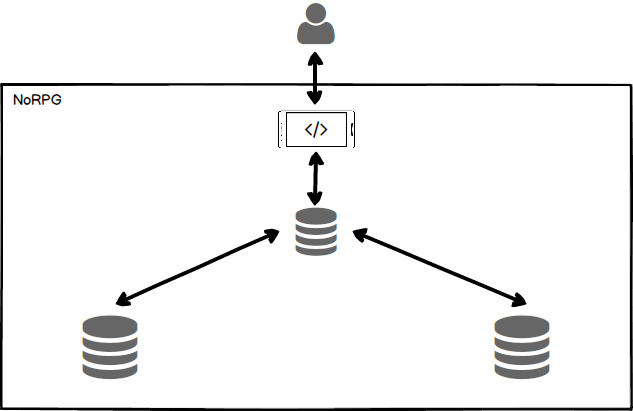
\includegraphics[width=12cm]{pics/HighLevelView.png}
			\captionof{figure}{High-Level-View von NoRPG} 
		\end{center}
		
		NoRPG besteht aus zwei Kernkomponenten. Die erste Kernkomponente ist die App, die aus der Graphical User Interface (GUI) und einer eingebetteten lokalen Datenbank besteht. Die zweite Kernkomponente ist eine Datenbank auf einem Server.
		
		Die Schnittstelle zwischen der App und dem Betriebssystem Android ist eine Systemschnittstelle. Systemschnittstellen identifizieren die Funktionalität der Software, um die Systemanforderung und die Schnittstellenbeschreibung zu erfüllen, damit die Software mit dem System übereinstimmt\footnote{vgl. Tripp \cite{srsIEEE}(1998) Seite 13}.
		
		Bei der Schnittstelle zwischen dem User und der Benutzeroberfläche der App handelt es sich um die Benutzerschnittstellen des Systems. Die Benutzerschnittstellen beschreiben die Kommunikation zwischen NoRPG und dem User. Der User kann mit NoRPG nur über die GUI der App interagieren.
		
		Jede Schnittstelle zwischen NoRPG und Hardwarekomponenten des Systems werden als Hardwareschnittstellen bezeichnet. Das Smartphone und seine Komponenten sind einzige Hardwarekomponente. Zu einem Smartphone gehört das Touchscreen, die Lautsprecher oder der WLAN-Adapter. Die Hardwarekomponente wird in der Abbildung durch das Smartphone dargestellt.
		
		Die App muss mit der lokalen und der serverseitigen Datenbank kommunizieren. Dabei handelt es sich um Softwareschnittstellen. Sie bilden den Übergang zwischen unterschiedlichen Programmen und ermöglichen dadurch das Nutzen derer Funktionalitäten. 

	\subsection{Produktfunktionen}
		In diesem Unterkapitel werden die wichtigsten Funktionen von NoRPG zusammengefasst. Das Ziel von NoRPG wie in Kapitel 2 schon beschrieben ist es, Lernspiele in einer festgelegten standardisierten Reihenfolge zum Herunterladen anzubieten. Dieses Ziel macht das Herunterladen von Spielen zu seiner Hauptfunktion. Um jedoch diese simple Funktionalität attraktiver zu gestalten, wird es die Funktion geben Collectables, zu Deutsch Sammelgegenstände, zu sammeln und mit Elementen im Spiel zu interagieren.
		
		Neben dieser Hauptfunktion gibt es weitere Produktfunktionen, um den Spieler zu identifizieren und das Spielerlebnis zu verbessern. Um den User zu identifizieren wird es eine Anmelde- und Registrierungsfunktion geben. In der Registrierung wird es möglich sein, einen personalisierten Charakter zu erstellen. 
		
		Im Spiel selbst wird es neben Spieloptionen wie Qualitäts- und Audioeinstellungen noch Features geben, die das Spielerlebnis verbessern. Der User wird in der Lage sein eine Karte von der Spielwelt zu öffnen, eine Liste von allen heruntergeladenen Spielen zu verwalten und seinen Fortschritt zu betrachten.
		
		Die App speichert den Fortschritt in der lokalen eingebetteten Datenbank und synchronisiert diese Daten, wenn eine aktive Internetverbindung besteht, mit der Datenbank auf dem Server.
	
	\subsection{Benutzermerkmale}
		In diesem Projekt wird zwischen zwei Benutzergruppen unterschieden.
		
		Die erste Benutzergruppe sind die User, viel mehr die Spieler. Grundsätzlich richtet sich NoRPG an Kinder, die keine Möglichkeit haben eine Schule zu besuchen. Jedoch werden keine Benutzergruppen für diese App ausgeschlossen. Egal ob jung oder alt, sowie männlich oder weiblich. Der Spieler sollte nur eine Neugier zum Lernen mitbringen. 
		
		Der Spieler benötigt Erfahrung mit der Verwendung eines Smartphones, insbesondere mit einem Android-Systems. Dazu zählt die Bedienung der Android-Oberfläche und die des Google Play Stores. Zudem sollten die User englische Texte verstehen können, da NoRPG zunächst nur in der englischen Sprache erscheinen wird.
		
		Die zweite Benutzergruppe sind die Administratoren.	Die Administratoren wollen Daten analysieren und daraus Aktionen ableiten. Für diese Benutzergruppe wird in diesem Projekt keine Benutzeroberfläche implementiert, jedoch wird eine Schnittstelle vorgesehen. 
			
	\subsection{Einschränkungen}
		Es wird zwischen Einschränkungen für die Entwickler und für die Spieler unterschieden.
		
		Entwickler müssen sich grundsätzlich zunächst an die regulatorischen Richtlinien, wie beispielsweise an die Datenschutzerklärung von Google oder an das IT-Sicherheitsgesetz halten.
		
		Da NoRPG sich an Kinder in bildungsfernen Ländern richtet ist es besonders wichtig, dass die Texte in NoRPG einfach zu verstehen sind. Da das Spiel zunächst nur in Englisch erscheinen wird, dürfen die englischen Texte kein Fachjargon oder ähnliches beinhalten. Die App darf keine hohen Mindestanforderungen an Hardwareressourcen haben, da der Smartphonestandard in bildungsfernen Ländern geringer ist. Das bedeutet für die Entwickler das Spiel so gut wie möglich Ressourcen-schonend umzusetzen. Des Weiteren gilt es bei der Implementierung zu beachten, dass NoRPG ohne eine aktive Internetverbindung soweit wie möglich spielbar bleiben muss.
		
		Allerdings gibt es auch Einschränkungen, die für die Spieler gelten oder zumindest temporär. Wie schon öfter erwähnt wurde, wird das Spiel zunächst nur in Englisch erscheinen. 
		
		Für die Anmeldung, die Registrierung, das Herunterladen von Spielen, das Synchronisieren und installieren von Updates wird eine aktive Internetverbindung vorausgesetzt. Des Weiteren benötigt der Spieler ein Android System, welches die Mindestanforderungen von NoRPG erfüllt.
				
	\subsection{Annahmen und Abhängigkeiten}
		Eine Annahme von NoRPG ist, dass es immer auf Smartphones, die genügend Leistung haben, verwendet wird. Wenn das Telefon nicht über genügend Hardwareressourcen für die Anwendung verfügt, kann es Szenarien geben, in denen die Anwendung nicht wie beabsichtigt oder überhaupt nicht funktioniert.
		
		Eine weitere Annahme ist, dass das Smartphone und dessen Hardware sowie Software funktionieren. Das Smartphone muss sich mit dem Internet verbinden können, wenn der Benutzer sich anmelden möchte oder Lernspiele herunterladen will. Neben einer funktionierenden Internetverbindung sollten andere Hardwareelemente wie die Lautsprecher oder der Touchscreen funktionieren. Das Smartphone muss eine gültige Android Version mit einem Google Konto besitzen.
		
	\subsection{Aufteilung der Anforderungen}
		In dem Fall, dass das Projekt verzögert wird, gibt es einige Anforderungen, die auf die nächste Version der Anwendung übertragen werden könnten.

\section{Spezifische Anforderungen}
	Das letzte Kapitel des SRS dient dazu alle Softwareanforderungen detailliert zu beschreiben. Dies ermöglicht es Designern ein System zu entwickeln, welches allen Anforderungen entspricht, und Testern, NoRPG ausreichend zu testen.
	
	\subsection{Externe Schnittstellen}
		Dieser Abschnitt ist die detaillierte Beschreibung aller Ein- und Ausgänge von NoRPG. Die Beschreibung ergänzt und vervollständigt die Schnittstellenbeschreibung von Kapitel 2.2.1. 
	
	%It should include both content and format as follows:
	%	a) Name;
	%	b) Beschreibung Zweck;
	%	c) Quelle des Inputs und Ziele des Outputs;
	%	d) Gültigkeitsbereich, Genauigkeit + Toleranz;
	%	e) Maßeinheit;
	%	f) Timing;
	%	g) Beziehungen zu anderen In-/Outputs;
	%	h) Screen(Bildschirm)format /-organisation;
	%	i) Fenster(Window)format /-organisation;
	%	j) Datenformat;
	%	k) Kommandoformat;
	%	l) End messages.
	
		\subsubsection{Systemschnittstellen}
			Name: Android 
			Beschreibung und Zweck: Betriebssystem des Smartphones
			Gültigkeitsbereich: Nur für die App von NoRPG
			Datenformat
			Kommandoformat
		
		\subsubsection{Benutzerschnittstellen}
			Die Benutzerschnittstellen, die user interfaces, sind der Punkt, an dem der Benutzer mit der Software interagiert. Zur Beschreibung der Benutzerschnittstellen werden logische Eigenschaften sowie Aspekte zur Optimierung formuliert. Zur Demonstration werden Mockups verwendet. Mockups stellen dar, wie die Oberfläche aussehen kann. Die am Projektende implementierte Oberfläche kann sich von den Mockups unterscheiden.
			
			Einem Benutzer, der NoRPG zum ersten Mal startet oder der nicht angemeldet ist, wird der Login-Screen präsentiert. Auf dem Login-Screen hat der Benutzer die Möglichkeit sich mit seinem Benutzernamen und seinem Passwort anzumelden oder sich, falls noch nicht geschehen, bei NoRPG zu registrieren. Das Smartphone muss Quer gehalten werden, da alle Elemente des Bildschirms vertikal angeordnet sind. Diese Eigenschaft trifft auch auf alle anderen Benutzerschnittstellen zu. Das Layout des Login-Screens ist ein Border-Pane, in dem die Bestandteile in einer einzigen Spalte angeordnet sind. Zur Optimierung der Nutzung werden kurze Fehlermeldungen ausgegeben, wenn der Benutzer falsche Login-Daten eingibt.
			\begin{center}
				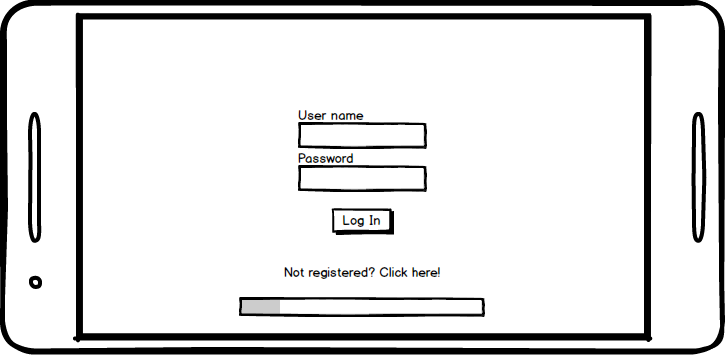
\includegraphics[width=10cm]{pics/Login.png}
				\captionof{figure}{Login-Screen Mockup} 
			\end{center}
			
			Falls sich der Benutzer bei NoRPG registrieren möchte, hat er die Möglichkeit dies in der App zu machen. Dazu klickt der Benutzer im Login-Screen auf den Register-Button. Anschließend öffnet sich der Register-Screen. Die Elemente sind im Tabellen Layout angeordnet, wodurch der Benutzer weiß, welche Daten in welches Feld eingetragen werden müssen. Die Registrierung ist notwendig, damit der Spielstand, somit der Fortschritt in einer Relation mit dem Benutzer steht. Zur weiteren Optimierung werden kurze Fehlermeldungen ausgegeben, damit ich der Benutzer weiß, in welchem Feld ein Fehler ist.
			
			\begin{center}
				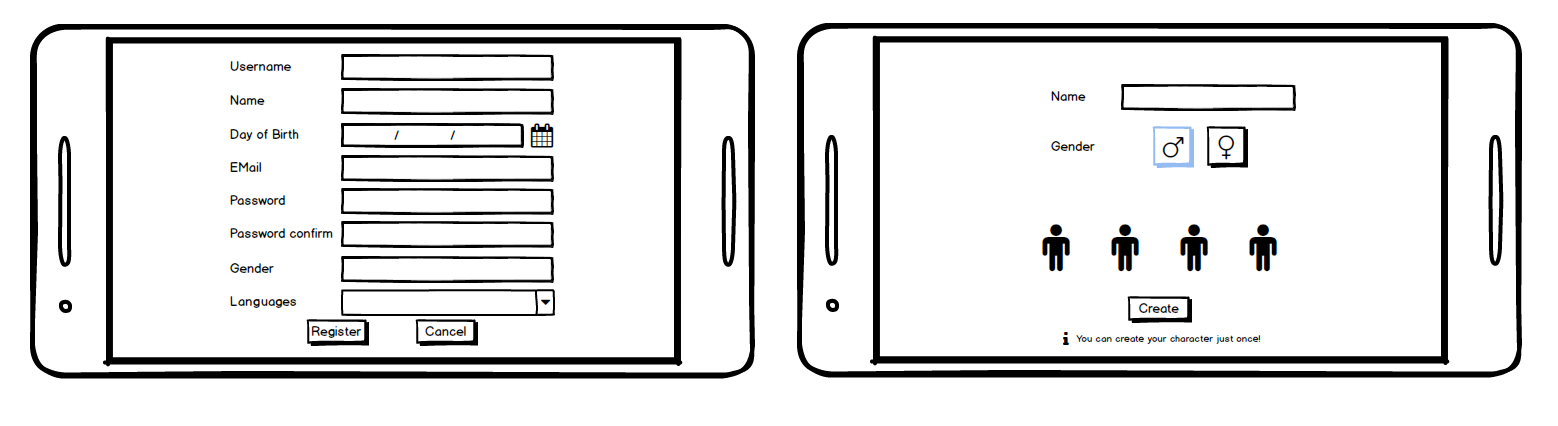
\includegraphics[width=\textwidth]{pics/Registerprozess.png}
				\captionof{figure}{Registerprozess: Registrierung und Create Character Mockup} 
			\end{center}
			
			Nach der Registrierung kann der Spieler einmalig seinen Charakter für den angelegten Account erstellen. Dazu bestimmt der Benutzer den Namen, das Geschlecht und das Aussehen des Charakters.
			
			NoRPG startet, nachdem alles geladen wurde und der Benutzer angemeldet ist. Das Spiele-Screen besteht aus der Spielewelt (Grafik) und dem Head-Up Display, kurz HUD. Das HUD ist eine Methode, mit der Informationen visuell als Teil der Benutzeroberfläche eines Spiels vermittelt werden. Während die Informationen, die auf dem HUD angezeigt werden, stark vom Spiel abhängen, gibt es viele Eigenschaften, die Spieler über viele Spiele erkennen. Die meisten von ihnen sind statisch auf dem Bildschirm, so dass sie während des Spiels sichtbar bleiben. 
			
			\begin{center}
				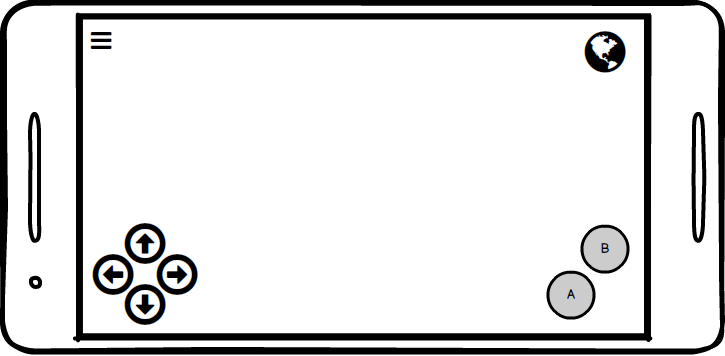
\includegraphics[width=10cm]{pics/HUD.png}
				\captionof{figure}{HUD Mockup} 
			\end{center}
			
			Das Mockup 3 enthält alle direkt sichtbaren HUD Elemente, die während des Spieles aktiv sind. Die Elemente sind an die Ecken gebunden, so befindeen sich beispielsweise die Pfeiltasten zur Bewegung des Charakters in der linken unteren Ecke des Bildschirms (siehe Graifk). Es sind so wenig Elemente wie möglich auf dem Bildschirm angeordnet und die verwendeten Symbole sind aus anderen bekannten Spielen und Konsolen übernommen und sind quasi ein Standard. Durch diese bekannte Anordnung der Elemente kann der User Informationen schneller verstehen und schneller reagieren. %vllt bisschen noch was zu dieser Anordnung labern
			
			Das Menü, welches sich in der oberen linken Ecke befindet, kann geöffnet werden. Dadurch wird das laufende Spiel pausiert und es werden weitere Optionen bzw. Interaktionen mit dem Spiel möglich. Diese HUD Elemente werden nur dann sichtbar, wenn der Spieler das Menü öffnet. Dadurch rückt das Spiel und die anderen Elemente in den Hintergrund. Das bedeutet nicht, dass die Elemente ausgeblendet werden, sondern dass der Benutzer diese Elemente nicht benutzen kann solange das Menü offen ist.
			
			\begin{center}
				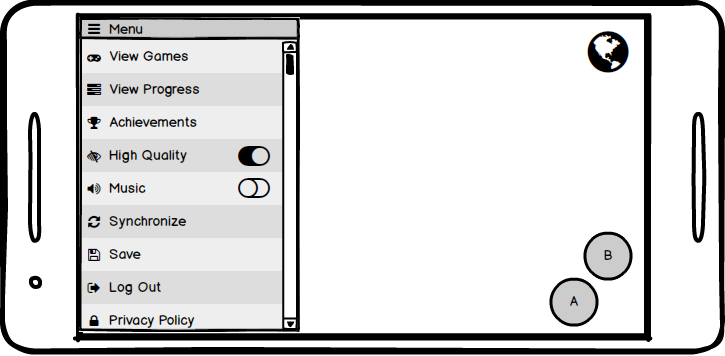
\includegraphics[width=10cm]{pics/Menu.png}
				\captionof{figure}{HUD offenes Menü Mockup} 
			\end{center}
			
			Einige der Menü-Elemente öffnen wiederum einen anderen Screen. Diese werden dann über das aktuelle Spiel geöffnet. Das Spiel befindet sich im Hintergrund und kann nicht gesehen bzw. angeklickt werden. Der neu geöffnete Screen muss erst geschlossen werden um das Spiel fortsetzen zu können. Ein Beispiel dafür ist der Fortschritt-Screen. Hier kann der Benutzer seinen Lern- bzw. Spielfortschritt betrachten.
			
			\begin{center}
				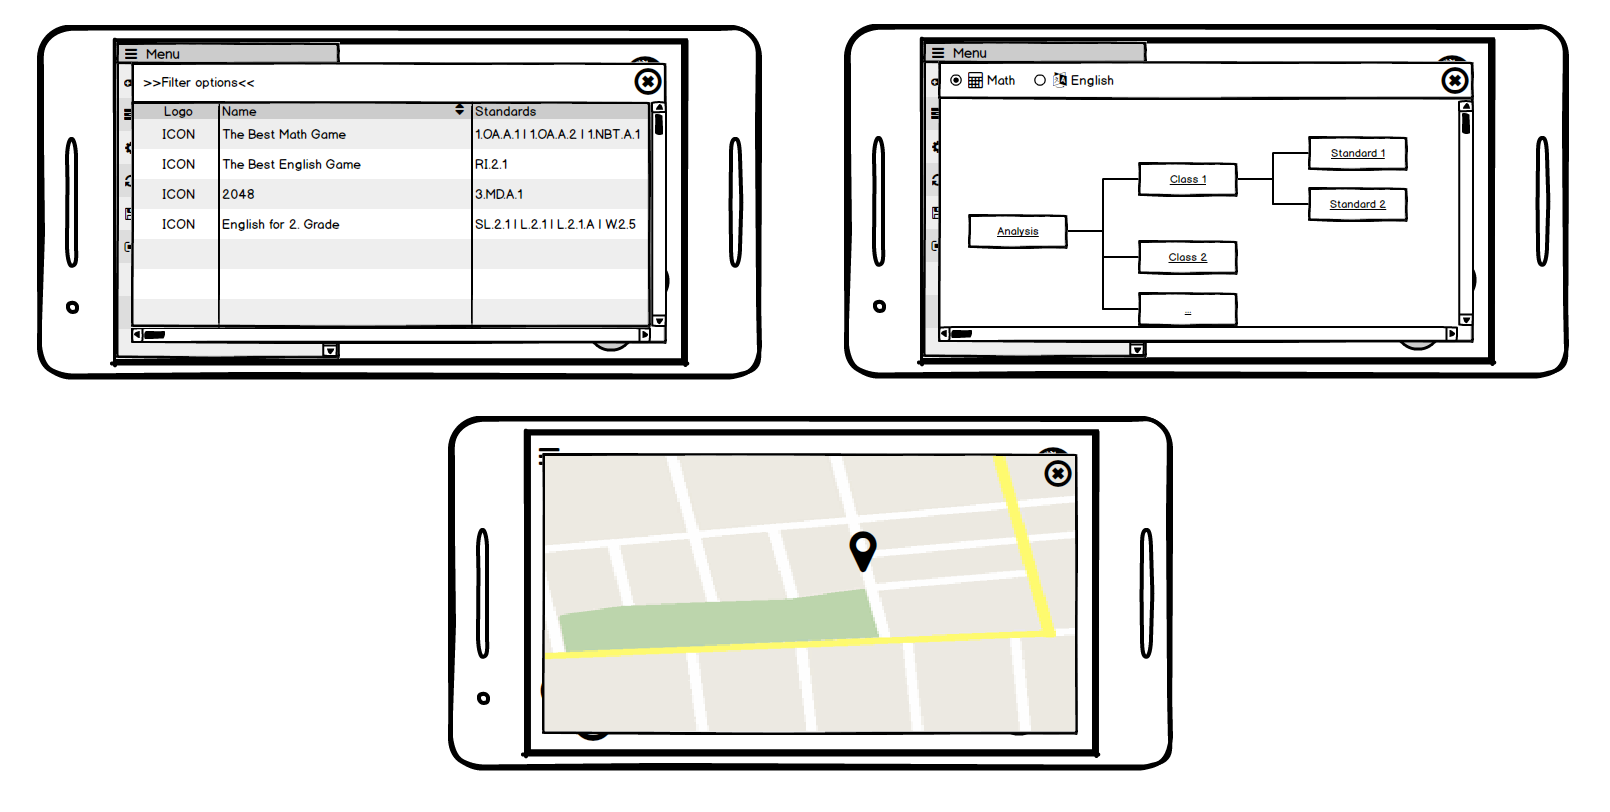
\includegraphics[width=\textwidth]{pics/NewWindows.png}
				\captionof{figure}{Spieleliste-, Fortschritt- und Karte-Fenster Mockup} 
			\end{center}
			
			Die Auflistung aller Screens würde den Rahmen dieser Arbeit überschreiten. Daher befinden sich die Mockups für die restlichen Screens im Anhang.
						
			%logische Eigenschaften:  required screen formats, page or window layouts, content of any reports or menus, or availability of programmable function keys
			
			%Aspekte Optimierung: comprise a list of do's and don'ts on how the system will appear to the user: long or short error messages
		
		\subsubsection{Hardwareschnittstellen}
			Die Hardwareschnittstellen spezifiziert die logischen Eigenschaften jeder Schnittstelle zwischen NoRPG und den Hardwarekomponenten des Systems. Die App hat eine  Hardwareschnittstelle mit dem Smartphone und seinen Komponenten.
			
			Ein Smartphone besteht aus sehr vielen Hardwarekomponenten. Jede einzelne Komponente wird benötigt, damit das Smartphone mit seinem kompletten Funktionsumfang funktioniert. Jedoch spielen einige Hardwarekomponenten eine besondere Rolle. Zu einem der Touchscreen eines Smartphones -> Toucheingaben für die Steuerung des Charakters, Interaktion mit dem Spiel, Menü, etc --> die einzige Benutzerschnittstelle
			
			WLAN-Adapter - verbindung mit dem Internet um mit dem Server zu kommunizieren
			
		\subsubsection{Softwareschnittstellen}
			This should specify the use of other required software products and interfaces with other application systems 
			
			Data mangement system, Google Play Store, 
			
			Software - Kommunikation mit GUI, kommunikation mit DB, ggf. logging

	\subsection{Funktionale Anforderungen}
		Use Cases dokumentieren Funktionalitäten eines Systems auf Basis von einfachen Modellen. In einem Use Case wird das nach außen sichtbare Verhalten eines Systems aus der Sicht der Nutzer beschrieben. Ein Nutzer kann hierbei eine Person, eine Rolle oder ein anderes System sein. Dieser Nutzer tritt als Akteur mit dem System in Interaktion, um ein bestimmtes Ziel zu erreichen. %quelle
		
		Use Cases verwenden Activity UML um anzuzeigen, wie der Benutzer vorgehen muss. Ein Aktivitätsdiagramm ist ein Verhaltensdiagramm der Unified Modeling Language (UML) und stellt die Vernetuzung von elementaren Aktionen und deren Verbindungen mit Kontroll- und Datenflüssen grafisch dar.
	
		\begin{center}
			
\includegraphics[width=10cm]{pics/OUCD.pdf}
			\captionof{figure}{Overall Use Case Diagramm} 
		\end{center}
		
		Das abgebildete System stellt die zu entwickelnde App für die User dar. Die App stellt die Graphische Oberfläche und somit die beschrieben Benutzerschnittstellen dar. Es sind nur die Funktionalitäten enthalten, die der Benutzer ausführen kann, also jene die über die Benutzerschnittstellen angesprochen werden können. Use Cases wie Login oder Registrierung sind im Overall Use Case Diagramm nicht enthalten, da diese im Vergleich zu anderen Use Cases primitiv sind. 
		
		Es werden nur die Use Cases des Players betrachtet, da die Use Cases des zweiten Benutzers, den Administratoren, zunächst nicht implementiert sondern nur entsprechende Vorkehrungen für die Implementierung getroffen werden.
	
		\subsubsection{Create character}
			Dieser Use Case beschreibt den Anwendungsfall, dass der Benutzer seinen Charakter erstellen möchte. Dieser Use Case wird pro Account genau einmal nach der Registrierung ausgeführt und zählt noch zum Prozess der Registrierung.
			
			Nach erfolgreicher Registrierung kann der Spieler seinen Charakter erstellen. Der User kann seinem Charakter einen Namen geben, das Geschlecht auswählen und anschließend das Aussehen bestimmen. Anschließend wird dem User der Hinweis angezeigt, dass es sich um eine einmalige Aktion handelt. Nachdem diese bestätigt wurde, wird der Charakter erstellt und gespeichert.
				
			\begin{center}
				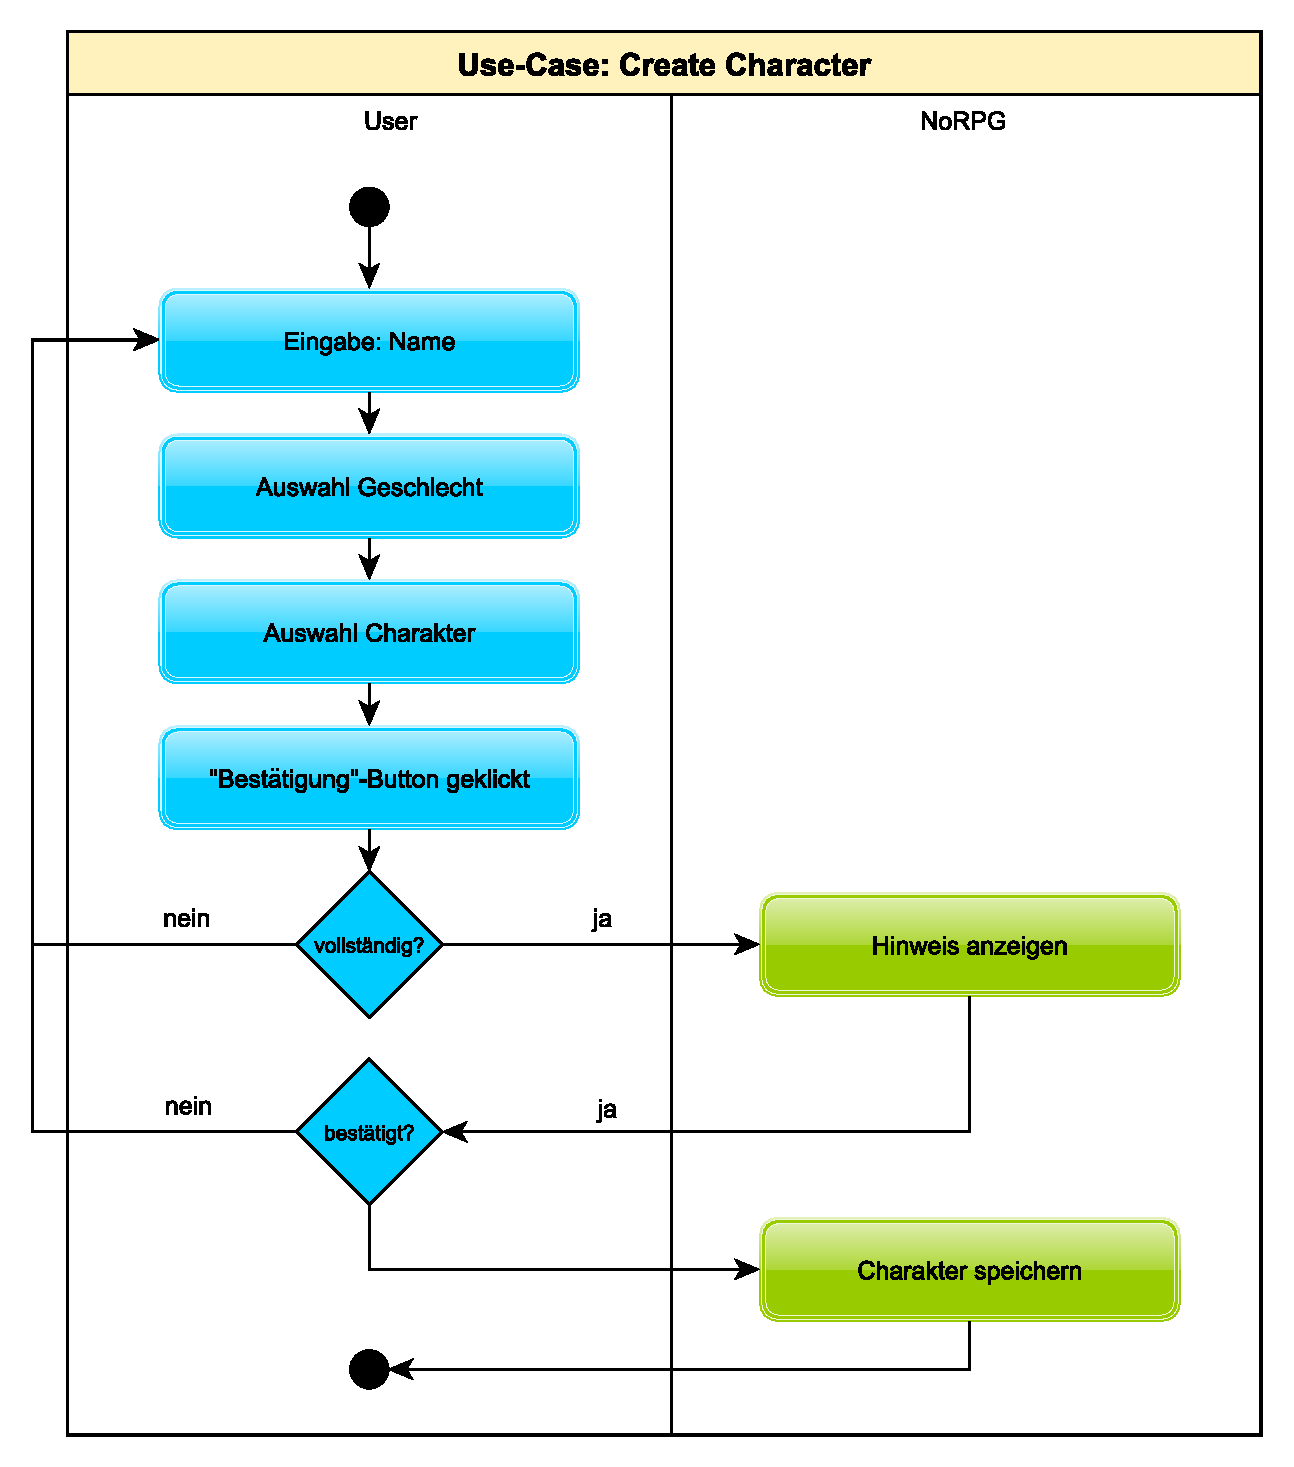
\includegraphics[width=10cm]{pics/CreateCharacter.pdf}
				\captionof{figure}{Create Character Activity UML} 
			\end{center}
	
			Bevor jedoch dieser Use Case ausgeführt werden kann, muss die Registrierung vollständig und erfolgreich abgeschlossen werden. Die Registrierung ist erfolgreich, wenn alle benötigte Daten eingetragen wurden und der Account noch nicht existiert. Für den gesamten Registrierungsprozess wird eine aktive Internetverbindung benötigt.
			
			Nach erfolgreicher Erstellung des Charakters, wird dieser in die Datenbank gespeichert und der User kann sich nun anmelden und in die Rolle seines Charakters schlüpfen.
			
		\subsubsection{Open map}
			Dieser Use Case beschreibt den Anwendungsfall, dass der Benutzer die Karte öffnet. Die Karte dient zur Orientierung der Welt und beinhaltet Symbole etc. um herauszufinden was so ist
			
			Ereignisablauf:	Benutzer öffnet Menü und klickt auf "Map" ...
	
			Vorbedingungen: Menü offen, Benutzer befindet sich nicht in einer NPC Interaktion
			
			Nachbedingungen: Eine Karte von der aktuellen Welt wird geöffnet
	
		\subsubsection{Show games}
			Dieser Use Case beschreibt den Anwendungsfall: Liste der gespielten und heruntergeladneen Spiele wird angezeigt. Zuordnung zu den Standards. Aus NoRPG das Spiel starten können.
			
			Ereignisablauf: Benuter öffnet Menü und klickt auf "Games" ...

			Vorbedingungen: Menü offen, Benutzer befindet sich nicht in einer NPC interaktion
			
			Nachbedingungen: Eine Liste wird angezeigt
	
		\subsubsection{View progress}
			Dieser Use Case beschreibt den Anwendungsfall, dass der Benutzer 
			
			Ereignisablauf
	
			Vorbedingungen
			
			Nachbedingungen
	
		\subsubsection{Settings}
			Dieser Use Case beschreibt den Anwendungsfall, dass der Benutzer 
			
			Ereignisablauf
	
			Vorbedingungen
			
			{Nachbedingungen
	
		\subsubsection{Synchronize}
			Dieser Use Case beschreibt den Anwendungsfall, dass der Benutzer 
			
			Ereignisablauf
	
			Vorbedingungen
			
			Nachbedingungen
	
		\subsubsection{Save local}
			Dieser Use Case beschreibt den Anwendungsfall, dass der Benutzer 
			
			Ereignisablauf
	
			Vorbedingungen
			
			Nachbedingungen
		
		\subsubsection{Character control}
			Dieser Use Case beschreibt den Anwendungsfall, dass der Spieler seinen Charakter in NoRPG durch die Spielwelt kontrolliert.
			
			Ereignisablauf
			
			Vorbedingungen: Spieler befindet sich im Spiel (nicht loading screen und menü ist geschlossen)
			
			Nachbedingungen: Charakter bewegt sich, bestätigt oder lehnt ab
	
		\subsubsection{game interaction}
			Dieser Use Case beschreibt den Anwendungsfall, dass der Benutzer sich in einer Interaktion mit einem NPC befindet. NPC bedeutet Non-Player Charakter und stellt die programmierten Charaktere dar (Unterhaltungen mit NPC, Storytelling)
			
			Ereignisablauf
			
			Vorbedingungen: Spieler befindet sich im Spiel (nicht loading screen und menü ist geschlossen)
			
			Nachbedingungen: Charakter bewegt sich, bestätigt oder lehnt ab
				
		%\begin{itemize}
		%	\item{Die Interaktion mit NPC's starten eine Unterhaltung, wodurch der Spieler mehr über das Spiel erfahren kann.}
		%	\item{Die Interaktion mit einer Verschlossenen Truhe zeigt die Lernspiele, die gespielt werden müssen um die Truhe öffnen zu können.}
		%	\item{Die Interaktion mit einer freigespielten True, ermöglicht dem Spieler die Truhe zu öffnen.}
		%	\item{Die Interaktion mit Collectables, die durch das Suchen/Reisen gefunden werden können, sammelt diese.}
		%	\item{Die Interaktion mit der Umwelt (Tiere, Bäume, etc.) startet keine Aktion.}
		%\end{itemize}
	
	\subsection{Performanz Anforderungen}
		This subsection should specify both the static and the dynamic numerical requirements placed on the software or on human interaction with the software as a whole. Static numerical requirements may include the following
		
		The number of terminals to be supported, The number of simultaneous users to be supported, Amount and type of information to be handled
		
	\subsection{Datenbank Anforderungen}
		This should specify the logical requirements for any information that is to be placed into a database. This may include the following:
		
		Types of information used by various functions
		
		Frequency of use
		
		Accessing capabilities
		
		Data entities and their relationships
		
		Integrity constraints
		
		Data retention requirements.
	
	\subsection{Entwurfsbeschränkungen}
		This should specify design constraints that can be imposed by other standards, hardware limitations, etc.
		
		Standards compliance: This subsection should specify the requirements derived from existing standards or regulations. They may include the following: 
		
		Report format, Data naming, Accounting procedures and Audit tracing.
		
		Als Maßstab werden dabei die Hardware des Smartphones Samsung Galaxy S4 genommen. Das Samsung Galaxy S4 kostet ungefähr 250€\footnote{Stand 04.01.2017 \url{https://www.amazon.de/Samsung-Smartphone-Touch-Display-Speicher-Android-Schwarz/dp/B00BTCE2M0}} und hat das Betriebssystem Android 5.0 Lollipop vorinstalliert und besitzt ausreichend gute Hardwarekomponenten. Die Auflösung des Displays mit 1080 x 1920 Pixel ist ausreichend, die 2 GByte Arbeitsspeicher sind notwendig und die 16 GByte interner Speicher sind ausreichend. Bei dem Prozessor handelt es sich um ein Qualcomm Snapdragon 600, mit vier Kernen und einer 32-bit Architektur\footnote{für mehr Informationen: \url{http://www.samsung.com/de/consumer/mobile-devices/smartphones/galaxy-s/GT-I9506ZKADTM}}.
	
	\subsection{Benuzterfreundlichkeit}
		Kindgerecht
		Einfach, simpel, nicht zu voll,
		
		Bsp: sichtbares Steuerkreuz anstatt Ziehfunktion wie bei anderen RPGs (vielleicht ein Bild hier um den Unterschied zu verdeutlichen)

	\subsection{Zuverlässigkeit}
		%This should specify the factors required to establish the required reliability of the software system at time of delivery.
		Alle implementierte Funktionen sollten zur Auslieferung korrekt und zuverlässig funktionieren. Dazu zählt auch, dass die Funktionen in vertretbaren Zeiten terminieren. Beispielsweise sollte die Anmeldung funktionieren, wenn der Spieler registriert ist und die richtigen Benutzerdaten eingegeben hat, oder die Benutzereingaben für die Charaktersteuerung sollen korrekt interpretiert werden.
		
		Eine besondere Wichtigkeit hat die Implementierung der in Kapitel 2 beschriebenen Common Core State Standards. Diese sind wichtig für die Reihenfolge der spielbaren Lernspiele, damit ein Spieler mit einem Skilllevel der ersten Klasse in Geometrie keine Lernspiele für die fünfte Klasse angezeigt kriegt. Erst dadurch wird gewährleistet und kann sichergestellt werden, dass der Spieler die Lerninhalte korrekt vermittelt kriegt.
	
	\subsection{Verfügbarkeit}
		%This should specify the factors required to guarantee a defined availability level for the entire system such as checkpoint, recovery, and restart. 
		
		Da bei jeder App eine lokale Datenbank mit vorhanden ist, muss der Server nicht ganze Zeit verfügbar sein. Das gilt jedoch nur für die Benutzer, die NoRPG schon heruntergeladen und sich registriert sowie angemeldet haben. Wenn diese Bedingungen erfüllt sind, wird der ganze Fortschritt lokal gespeichert werden und kann mit dem Server manuell oder vor dem Ausloggen automatisch synchronisiert werden, muss es allerdings nicht. Denn der Server ist da, falls der User sich an einem anderen Gerät anmelden möchte, dass der Spielstand dort gleich ist. 
		
		System Availability: MUST: 98\%, PLAN: 99\% und WISH: 100\%
		
		Server Availability: MUST: 80\%, PLAN: 99\% und WISH: 100\%
		
		Internet Connection: Die App sollte mit dem Internet verbunden sein, jedoch muss es nicht
		
	\subsection{Sicherheit}
		Bei Sicherheit wird zwischen zwei unterschiedlichen Typen unterschieden: Security und Safety. Security ist der Schutz vor absichtlichen Bedrohungen, wenn ein Angreifer absichtlich das Systems angreift. Im Gegensatz dazu ist Safety der Schutz vor unbeabsichtigten Bedrohungen, wenn der Benutzer durch Zufall die Sicherheitsmechanismen umgeht indem er etwas nicht beabsichtigtes ausführt.
		
		Die Kommunikation mit dem Server und mit der lokalen eingebetteten Datenbank müssen verschlüsselt werden, damit die Credentials bei den Anmeldung oder bei der Registrierung nicht mitgelesen werden können. Des Weiteren müssen die Daten auf der lokalen Datenbank validiert werden, bevor der Server synchronisiert wird, denn es wird unter anderem auch der Spielfortschritt der Benutzer synchronisiert. Die Veränderung des Spielfortschritts wird als Schummeln bzw. Cheaten behandelt.
		
		Die Anmeldung bzw. Registrierung ist notwendig, um NoRPG spielen zu können. Deswegen müssen die Accounts der Benutzer verschlüsselt gespeichert werden und die Passwörter dürfen bei der Anmeldung nur mittels One-Way-Functions vergleichen werden. Nicht registrierte bzw. unautorisierte Benutzer erlangen keinen Zugriff auf das System.
		
		Die gespeicherte Daten dürfen an andere Tools nur anonymisiert weitergegeben werden, für beispielsweise Analysezwecke. Diese Kommunikation mit anderen System oder Applikationen darf nur verschlüsselt geschehen.
		
	\subsection{Wartbarkeit}
		Der Code von NoRPG sollte so geschrieben werden, dass der Code die Umsetzung neuer Funktionen begünstigt. Deshalb sollte die Komplexität des Codes so gering wie möglich gehalten werden, indem entsprechende Methoden wie das Model-View-Controller Pattern umgesetzt werden. Des Weiteren sollte das System von NoRPG Schnittstellen jeglicher Art anbieten, um das System durch weitere Komponenten wie ein Web-Tool für Administratoren zu erweitern.
		
		Neben der Erweiterbarkeit sollte NoRPG für Fehlerfälle eine Testumgebung anbieten, um das Testen der Anwendung auf unterschiedliche Funktionen zu ermöglichen und gegebenenfalls Fehler wiederholen und simulieren zu können.
		
	\subsection{Portabilität}
		Die App NoRPG ist zunächst nur für Android geplant. Andere Betriebssysteme, wie Windows Phone von Microsoft oder iOS von Apple, sind vorerst nicht vorgesehen. 
		
		Bei der vorhanden Breite an Varianten von Android-Smartphones ist sehr wichtig, dass die Portabilität innerhalb von Android Smartphones gewährleistet wird. Neben bekannten Smartphoneherstellern wie Samsung, LG oder HTC gibt es zahlreiche weitere Hersteller die auf das Android Betriebssystem setzen. Jeder Hersteller hat dabei eine große Palette an Smartphone-Modellen, wie bei Samsung die Samsung Galaxy S-Reihe, welches aktuell in der siebten Genration erhältlich ist\footnote{Vgl. \url{http://www.computerbild.de/artikel/cb-News-Handy-Samsung-Galaxy-S-S2-S3-S4-S5-S6-S7-11332036.html}}, oder die Samsung Galaxy Note-Reihe. Die App NoRPG muss auf allen Android-Smartphones funktionieren, solange diese die Mindestanforderungen an Software und Hardware erfüllen. Dabei muss sich die App beispielsweise an die Auflösung oder XXX anpassen.
		
		Die Portabilität beschreibt nicht nur die technische Sicht sondern auch in welchen Ländern und in welchen Sprachen NoRPG verfügbar sein wird. Der Release findet in allen Ländern statt, in denen der Google Play Store verfügbar ist. Zunächst wird NoRPG nur in Englisch verfügbar sein, welches jedoch kein weiteres Problem darstellt.
\chapter{Umsetzung}

Nachdem im vorherigen Kapitel die technischen Grundlagen erläutert wurden, wird jetzt auf die Umsetzung eingegangen. Dabei wird diese in drei Teile unterteilt

\section{App}
Google Anmeldung wird nicht genutzt, da wir nur ein paar spezielle Informationen von den Spielern brauchen und Google Daten geben??
Vorteil an Android und Google Play Store: Google Play Store: große Anzahl an vielfältigen Apps, Schutz durch Google Play, da Apps Kriterien erfüllen müssen um aufgenommen zu werden

		Durchführen von Usability-Tests

\section{Datenbank auf dem Handy}
Wieso haben wir das gemacht? Vorteile? Nachteile?
Speicherung von Daten --> wieso nicht PlayerPrefs von Unity benutzen sondern Serialisieren? Doku, Paper, ... begründen und Beispiel zeigen. Gespeichert wird in einer .dat anstatt .txt, nicht einfach lesbar bearbeitbar (daten lesen etc.)
	
\section{Datenbank auf dem Server}
Bei der Datenbank auf dem Server handelt es sich um eine MySQL Datenbank. In dieser sind die Daten der Registrierten User und deren Fortschritt in den Tabellen accounts und spielfortschritt gespeichert.

\section{C\# Skripte}

Nachfolgend wird auf die einzelnen C\# Skripte eingegangen, welche für die App benötigt werden. Darüber hinaus wird auf weitere, für die Skripte essentielle umgesetzte Teile der App eingegangen.

\subsection{Player}

Der Player setzt sich aus mehreren einzelnen Objekten zusammen, darunter die Textur für den Spieler, ein Teil deiner Minimap und ein weiteres leeres Objekt, welches für die Kamera wichtig ist. An dem Player selbst befinden sich wiederum die Skripte und von Unity vorgefertigten Objekte. Ein sogenannter Rigedbody sorgt dafür, dass der Player Gravitation erfährt und nicht einfach durch die Luft schweben kann. Ein Character Controller fügt Eigenschaften wie eine Größe und höhe ein. Darüber hinaus besitzt der Player einen Animatoir. Dieser ist zusammen mit dem ThirdPersonController dafür verantwortlich, dass sich der Player in der Szene bewegt und die Animationen korrekt ausgeführt werden. Damit dies passiert, wird diesem Controller der Wert speed und direction übergeben. Daraus resultieren folgene Möglichkeiten der Animation

 \begin{table}[htpb]
 \begin{tabular}{|l|l|l|}
 \hline
  speed & direction & Ergebnis \\
 \hline
  0 & 0 & Animation Idle \\
  >0 & 0 & Animation Walk \\
  >0 & 0.3 & Animation Walk Right Short \\
  >0 & 0.5 & Animation Walk Right Medium \\
  >0 & -0.3 & Animation Walk Left Short \\
  >0 & -0.5 & Animation Walk Left Medium \\
  >0.5 & 0 & Animation Run \\
  >0.5 & 0.3 & Animation Run Right Medium \\
  >0.5 & 0.5 & Animation Run Right Wide \\
  >0.5 & -0.3 & Animation Run Left Medium \\
  >0.5 & -0.5 & Animation Run Left Wide \\ \hline
 \end{tabular}
  \caption{Mögliche Animationen je nach Wert speed und direction}
 \label{tab:tabspeeddirection}
 \end{table}
 
Durch diese vielzahl an Animationen ist gewährleistet, dass der Player zu jeder Zeit die richtige Animation ausführt und die Bewegung nicht unnatürlich aussieht. Die Werte speed und direction für diese Animation kommen dabei aus dem Skript CharacterControll.cs . Diese ist für die Steuerung des Players zuständig. Hier wird die Toucheingabe über den Joystick in Weltkoordinaten umgewandelt und der Player beginnt sich zu bewegen. Dazu ist die Update Methode genutzt worden. In dieser wird, sofern ein Animator an dem Player vorhanden ist, die horizontale und vertikale Bewegung des Joysticks in die direction und den speed umgewandelt. Das ganze passiert dabei in der Methode StickToWorldspace, welche die Transform vom Player, der Kamera, die direction und den speed, übergeben bekommt. Nachdem die Methode aufgerufen wurde und abgeschlossen ist, werden die Werte von direction und speed an den ThridPersonController übergeben und die Animation startet, wie zuvor beschrieben.

In der StickToWorldspace Methode wird zu Begin die rootDirection gesetzt, welche sich dabei aus der Z-Achsen Koordinate zusammensetzt. Anschließend wird die stickDirection gesetzt, durch den horizontalen und vertikalen Wert des Joysticks. Nun wird durch das quadrieren der beiden Werte der speed berechnet. Dieser liegt dabei zwischen Null und Eins.

Danach das ganze in bezug zu der Positionsrichtung der Kamera gesetzt, um die Bewegungsrichtung zu erhalten, um anschließend das Kreutzprodukt aus diesen beiden Werten zu berechen. Mit hilfe dessen kann bestimmt werden, ob sich der Player nach Rechts oder nach Links bewegen soll.

\begin{scriptsize}
\lstset{
	float,
	caption=Skript CharacterController.cs, 
	language=[Sharp]C, 
	frame=single,  
	showstringspaces=false, 
	showspaces=false, 
	numbers=left, 
	captionpos=b, 
	belowcaptionskip=4pt,
	basicstyle=\ttfamily
} 
\newpage
\begin{lstlisting}[label=lst:c_charactercontroller]
using UnityEngine;
using CnControls;
using UnityStandardAssets.CrossPlatformInput;
using UnityEngine.SceneManagement;

public class CharacterControll : MonoBehaviour {

	...

    private float speed = 0.0f;
    private float direction = 0f;
    private float horizontal = 0.0f;
    private float vertical = 0.0f;
    private AnimatorStateInfo stateInfo;

	...	
	
    void FixedUpdate() {
        if(IsInLocomotion() && ((direction>=0 && horizontal>=0) 
        	|| (direction <0 && horizontal < 0))) {
        	
            Vector3 rotationAmount = Vector3.Lerp(Vector3.zero, new Vector3(0f, 
            rotationDegreePerSecound * (horizontal < 0f ? -1f : 1f), 0f), 
            Mathf.Abs(horizontal));
            	
            Quaternion deltaRotation = Quaternion.Euler(rotationAmount * Time.deltaTime);
            this.transform.rotation = (this.transform.rotation * deltaRotation);
        }
    }

    public bool IsInLocomotion() {
        return stateInfo.nameHash == m_LocomotionID;
    }

    void Update() {
    
        if (animator) {
            stateInfo = animator.GetCurrentAnimatorStateInfo(0);
            horizontal = CnInputManager.GetAxis("Horizontal");
            vertical = CnInputManager.GetAxis("Vertical");
            StickToWorldspace(this.transform, gamecam.transform, ref direction, ref speed);
            animator.SetFloat("speed", speed);
            animator.SetFloat("direction", direction, directionDumpTime, Time.deltaTime);
        }
    }
    
    ...

    public void StickToWorldspace(Transform root, Transform camera, 
    	ref float directionOut, ref float speedOut) {
    	
        Vector3 rootDirection = root.forward;
        Vector3 stickDirection = new Vector3(horizontal, 0, vertical);
        speedOut = stickDirection.sqrMagnitude;
        Vector3 CameraDirection = camera.forward;
        CameraDirection.y = 0.0f;
        Quaternion referentialShift = Quaternion.FromToRotation(Vector3.forward, 
        	Vector3.Normalize(CameraDirection));
        	
        Vector3 moveDirection = referentialShift * stickDirection;
        Vector3 axisSign = Vector3.Cross(moveDirection, rootDirection);
        float angleRootToMove = Vector3.Angle(rootDirection, moveDirection) * 
        	(axisSign.y >= 0 ? -1f : 1f);      
        	
        angleRootToMove /= 180f;
        directionOut = angleRootToMove * directionSpeed;
    }
}

\end{lstlisting}
\end{scriptsize}

\subsection{Kamera}



\subsection{Portale}



\subsection{Minimap}



\subsection{Interaktionsmöglichkeiten}
Chests, Händler, etc....


\subsection{Pfadfindungssystem Schiff}
Die tropischen Inseln von Galapagos werden im Spiel mit einem Schiff bereist. Dabei kann der Spieler aus fünf verschiedenen Inseln auswählen, und je nach Insel fährt das Schiff einen anderen Pfad. Diese Pfade sind dabei statisch und festgelegt. Es gibt dabei 20 Pfade, vier von jeder Insel. Jeder dieser Pfade ist ein Gameobject mit dem Skript EditorPathScript. (siehe Listing \ref{lst:c_patheditor})

\begin{scriptsize}
\lstset{
	float,
	caption=Skript EditorPathScript.cs, 
	language=[Sharp]C, 
	frame=single,  
	showstringspaces=false, 
	showspaces=false, 
	numbers=left, 
	captionpos=b, 
	belowcaptionskip=4pt,
	basicstyle=\ttfamily
} 
\newpage
\begin{lstlisting}[label=lst:c_patheditor]

using System.Collections;
using System.Collections.Generic;
using UnityEngine;

public class EditorPathScript : MonoBehaviour {

    //Color of the lines betwwen the single points
    public Color rayColor = Color.white;
    //List of all points of the path
    public List<Transform> path_objs = new List<Transform>();
    //List of all transformobjects of every point in path
    Transform[] transforms;

    //Method to draw in the Unity Editor
    void OnDrawGizmos () {
        //Set Color of lines to selected color
        Gizmos.color = rayColor;
        //Get all transformobjects of childrends
        transforms = GetComponentsInChildren<Transform>();
        //Clear the list
        path_objs.Clear();

        //Foreach transformobject at it to list if it is not the parentobject
        foreach (Transform path_obj in transforms) {
            if (path_obj != this.transform) {
                path_objs.Add(path_obj);
            }
        }
        //Draw lines between every Point
        for(int i = 0; i < path_objs.Count; i++) {
            Vector3 position = path_objs[i].position;
            if (i > 0) {
                Vector3 previos = path_objs[i - 1].position;
                Gizmos.DrawLine(previos, position);
                Gizmos.DrawWireSphere(position, 0.3f);
            }
        }
    }
}

\end{lstlisting}
\end{scriptsize}

Dieses sorgt dafür, das die Pfade grafisch im Unity Editor angezeigt werden. Dieses Skript zeichnet dabei von einem Startpunkt zum nächsten eine Linie, solange, bis der letzte Punkt erreicht wird. Dadurch wird es möglich die Pfade grafisch zu bearbeiten und erleichtert so die Arbeit. 
Nun wird beschrieben, wie das Schiff dem Pfad folgt, sobald der Player den Pfad ausgewählt hat. Dabei wird auf den Pfad von Insel eins zu zwei eingegangen. Für alle anderen Pfade ist das vorgehen identisch.

Über ein Userinterface wählt der Player den betroffenen Pfad aus. Dabei wird dieser über einen Button ausgewählt. Sobald dieser geklickt wurde wird eine Funktion in Listing \ref{lst:methode} ausgeführt. Diese selektiert den gewünschten Pfad aus den verfügbaren Pfaden und setzt den boolean playerOnShip auf true. 

\begin{scriptsize}
\lstset{
	float,
	caption=Methode selectFirstClass, 
	language=[Sharp]C, 
	frame=single,  
	showstringspaces=false, 
	showspaces=false, 
	numbers=left, 
	captionpos=b, 
	belowcaptionskip=4pt,
	basicstyle=\ttfamily
} 
\begin{lstlisting}[label=lst:methode]

public void selectFirstClass () {
//if player is not on the same Island
 if (lastButtonClicked != "1") {
  hud.SetActive(false);
  // set path to the island on that the player is to island 1
  path = GameObject.Find("Path" + lastButtonClicked + "_1").GetComponent<EditorPathScript>();
  lastButtonClicked = "1";
  playerOnShip = true;
 }
}

\end{lstlisting}
\end{scriptsize}

Da dieser boolean nun auf true gesetzt ist, wird der Code der Methode playerGetOnShip ausgeführt. Der Code ist in Listing \ref{lst:methode1} zu sehen. Durch diese Methode bewegt sich der Player mit dem Schiff in der selben Geschwindigkeit. Darüberhinaus blokiert diese Funktion die Eingabemöglichkeiten des Players während der Fahrt.

\begin{scriptsize}
\lstset{
	float,
	caption=Methode playerGetOnShip, 
	language=[Sharp]C, 
	frame=single,  
	showstringspaces=false, 
	showspaces=false, 
	numbers=left, 
	captionpos=b, 
	belowcaptionskip=4pt,
	basicstyle=\ttfamily
} 
\begin{lstlisting}[label=lst:methode1]

public void playerGetOnShip () {
 if (!playerOnShip) {
  cc.enabled = false;

  player.GetComponent<Animator>().SetFloat("speed", 0.0f);
  player.GetComponent<Animator>().SetFloat("direction", 0.0f);
  player.transform.position = ship.transform.position;

  player_mesh.SetActive(false);
  player_text.SetActive(false);

  follow.transform.parent = ship.transform;
  follow.transform.position = ship.transform.position + new Vector3(2.25f, 18.07f, -7.07f);

  minidot.SetActive(false);

  hud.SetActive(true);
 }
}

\end{lstlisting}
\end{scriptsize}

Des Weiteren wird die Funktion moveShip ausgeführt. Diese ist für die eigentliche Bewegung des Schiffes verantwortlich. Sobald playerOnShip auf true gesetzt ist, wird zuerst die Distanz zwischen dem ersten Punkt des Pfades und des Schiffes gespeichert und die Position des Schiffes an diese stelle verschoben. Anschließend wird die drehung des Schiffes an die Fahrtrichtung angepasst und gedreht. Sobald die Distanz zwischen der aktuellen Position des Schiffes und dem nächsten Punkt des Pfades kleiner ist wie eine minimale Distanz, wird die currentWayPointId um eins erhöhrt. Solange dieser Wert nicht größer ist wie die Anzahl der Punkte des Pfades werden diese Schritte wiedserholt und das Schiff bewegt sich entlang des Pfades.

\begin{scriptsize}
\lstset{
	float,
	caption=Methode moveShip, 
	language=[Sharp]C, 
	frame=single,  
	showstringspaces=false, 
	showspaces=false, 
	numbers=left, 
	captionpos=b, 
	belowcaptionskip=4pt,
	basicstyle=\ttfamily
} 
\begin{lstlisting}[label=lst:methode2]

public void moveShip () {
 //if player is on the ship
 if (playerOnShip) {
  //get the distance between ship and the first point
  float distance = Vector3.Distance(path.path_objs[currentWayPointId].position, transform.position);
  //set the ship to the first point
  transform.position = Vector3.MoveTowards(transform.position, path.path_objs[currentWayPointId].position, Time.deltaTime * speed);
  //set the player on ship
  player.transform.position = transform.position;

  //rotate the ship in direction to the next point
  var rotation = Quaternion.LookRotation(path.path_objs[currentWayPointId].position - transform.position);
  transform.rotation = Quaternion.Slerp(transform.rotation, rotation, Time.deltaTime * rotationSpeed);
  player.transform.rotation = ship.transform.rotation;

  //if the distance between the ship and the point is less then reachDistance raise the currentwaypointid
  if (distance <= reachDistance) {
   currentWayPointId++;
  }

  //if the currentwaypoint is greater equal the size of the list
  if (currentWayPointId >= path.path_objs.Count) {
   //set ship to the last position
   this.transform.position = path.path_objs[path.path_objs.Count-1].position;
   //set playershipped status to true and make some other things
   playerShipped = true;
   cc.enabled = true;
   playerOnShip = false;
   player_mesh.SetActive(true);
   player_text.SetActive(true);
   follow.transform.parent = player.transform;
   follow.transform.position = player.transform.position;

   minidot.SetActive(true);
   player.transform.position = new Vector3(path.path_objs[path.path_objs.Count - 1].position.x, 6.3f, path.path_objs[path.path_objs.Count - 1].position.z);
                
   currentWayPointId = 0;
  }
 }
}
    
\end{lstlisting}
\end{scriptsize}

\subsection{Datenimport aus JSON}

Der Datenimport aus einer JSON-Datei wird genau zwei mal im Spiel verwendet. Die Standarts und die Texte der NPCs stehen in JSOn-Notation bereit. Dabei werden beide Dateien unterschiedlich ausgelesen und genutzt. Zuerst wird auf die Standarts eingegangen und anschleißend auf die Verarbeitung der Datei mit Text. 

\subsubsection{Standarts JSON}
Die JSON für die Standarts ist ein wichtiger Bestandteil des Spieles. In dieser Datei befinden sich alle wichtigen Infos zu den Standarts und deren dazugehörigen Spiele. Diese Datei liegt Zentral auf einem Server und kann dort gewartet und gepflegt werden. Dadurch ist es möglich, zusätzliche Standarts und Spiele einzufügen, ohne das der Nutzer die App aktuallisieren muss. Nun wird der grobe Ablauf, gefolgt von einer detailierten Beschreibung, erklärt und beschrieben.

Damit der Nutzer die aktuelle Datei zur Verfügung hat, versucht das Spiel eine zu Beginn eine Verbindung zu dem Server aufzubauen. Gelingt dies, wird die Datei von Server geladen und auf dem Handy gespeichert. Nachdem die Datei gespeichert wurde, wird sie in das Spiel geladen. Dazu wird aus dem JSON eine Liste erstellt, welche überall im Spiel nutzbar ist.

Für das Laden und verarbeiten sind fünf Klassen verantwortlich. Im Folgenden wird nur deatiliert auf die Klasse WebJSONConfigReader eingegangen. Die anderen Klassen sind im Anhang abgebildet und werden nur erwähnt.

Die Klasse MappingStandardsToCourses ist die Datenhaltungsklasse. In dieser ist die Struktur der einzelnen Objekte geregelt. In der Klasse MappingStandardsToCoursesBean spiegelt die Struktur der JSON-Datei wieder. 

Der WebJSONConfigReader wird in der Klasse LoadingScreen genutzt. Dort wird eine Instanz dieser Klasse erzeugt und es wird die Methode LoadSettings ausgeführt und in der Variable Settings gespeichert. Diese Methode ist in Listing \ref{lst:methode3} zu sehen.


\begin{scriptsize}
\lstset{
	float,
	caption=Methode LoadSettings, 
	language=[Sharp]C, 
	frame=single,  
	showstringspaces=false, 
	showspaces=false, 
	numbers=left, 
	captionpos=b, 
	belowcaptionskip=4pt,
	basicstyle=\ttfamily
} 
\begin{lstlisting}[label=lst:methode3]

public MappingStandardsToCourses LoadSettings() {

 WWW www = new WWW(settingsURL);
 while (!www.isDone) { }
  string json;
  string LocalFilePath = Application.persistentDataPath + "/v1.json";

  if (string.IsNullOrEmpty(www.error)) {
   json = www.text;
   File.WriteAllText(LocalFilePath, json);
  } else if (File.Exists(LocalFilePath)) {
   json = File.ReadAllText(LocalFilePath);
  } else {
   json = "";                
   File.WriteAllText(LocalFilePath, json);
  }
  Debug.Log(json.ToString());
  MappingStandardsToCoursesBean settingsBean = MappingStandardsToCoursesBean.CreateFromJSON(json);
  string json2 = JsonUtility.ToJson(settingsBean);
  Debug.Log(json2.ToString());

  List<Classes> classes = new List<Classes>();
  foreach (var classe in settingsBean.classes) {
   List<Courses> courses = new List<Courses>();
   foreach (var course in classe.courses) {
    List<Standards> standards = new List<Standards>();
    foreach (var standard in course.standards) {
     List<Games> games = new List<Games>();
     List<string> vor = new List<string>();
     List<string> nach = new List<string>();
     foreach (var game in standard.games) {
      games.Add(new Games(game.id, game.name, game.url));
     }
     foreach (var vorbedingung in standard.vorbedingungen) {
      vor.Add(vorbedingung);
     }
     foreach (var nachbedingung in standard.nachbedingungen) {
      nach.Add(nachbedingung);
     }
     Games[] g = games.ToArray();
     string[] v = vor.ToArray();
     string[] n = nach.ToArray();
     standards.Add(new Standards(standard.name, v, n, g));
    }
    Standards[] s = standards.ToArray();
    courses.Add(new Courses(course.name, s));
   }
   Courses[] c = courses.ToArray();
   classes.Add(new Classes(classe.name, c));
  }
  Classes[] cla = classes.ToArray();
  return new MappingStandardsToCourses(cla);
 }
\end{lstlisting}
\end{scriptsize}

In dieser wird zu Beginn ein neues WWW Objekt erstellt. Dieses baut eine Verbindung zum Server auf. Anschließend wird in Zeile 9 überprüft, ob es zu einem Fehler beim Verbindungsaufbau gekommen ist. Wenn es zu keinem Fehler gekommen ist, wird der Inhalt des WWW Objekts in eine Datei geschrieben und gespeichert. Für den Fall das ein Fehler aufgetretten ist und das WWW Objekt keine Verbindung zum Server aufgebaut werden kann, wird geprüft ob bereits eine ältere Datei vorhanden ist, wenn ja, wird der Text aus dieser Datei zum Erzeugen des Objektes genutzt. Anschlißend wird in Zeile 19 aus dem Text eine JSON Struktur erzeugt. Aus dieser wird anschließend in mehreren Schritten ein mehrdimensionaler Array erzeugt und zurückgegeben.
\subsubsection{NPCText JSON}

\subsection{Datenimport aus / in Datenbank}

Zum Senden der Daten der Registrierung wird das Skript SendDataToServer.cs genutzt. In diesem werden die Daten der Registrierung zwischengespeichert und am Ende an den Server gesendet. Dazu wird die Methode SendRegister() genutzt. In dieser wird die Methode RegisterUser() als Coroutine gestartet. Dazu werden zehn Parameter übergeben, der Username, die Email, das Passwort, der Vorname, der Nachname, das Geburtsdatum, das Geschlecht, der Herkunftsstaat, die native Sprache und der gewählte Charakter. Bei einer Coroutine handelt es sich um einen Thread, welcher beliebig gestarte, pausiert und beendet werden kann.

Innerhalb dieser Methode wird zu Beginn ein Hash erstellt, welcher am Server genutzt wird, um zu überprüfen, ob die Anfrage gültig ist. Dieser besteht dabei aus teilen der Eingabe und einem zusätzlichen geheimen Schlüssel, welchem nur der App und dem Server bekannt sind. Dadurch wird die Sicherheit gesteigert und es wird Angreifern erschwert unberechtigte Zugriffe auf die Datenbank zu tätigen. Bei dm Hash handelt es sich dabei um die MD5 verschlüsselten Eingabedaten. Dadurch ist es fast nicht möglich, einen Validen Hash zu bilden, ohne diese Daten zu kennen.

Nachdem der Hash erstellt wurde, werden alle Parameter in Form einer Url aneinander gehängt. Anschließend wird die URL an ein WWW Objekt übergeben und solange gewartet, bis es eine Antwort gibt. Sofern es keinen Fehler gab, wird ein Text ausgegeben, welche vom Server gesendet wird, andernfalls eine Fehlermeldung.


\begin{scriptsize}
\lstset{
	float,
	caption=Skript SendDataToServer.cs, 
	language=[Sharp]C, 
	frame=single,  
	showstringspaces=false, 
	showspaces=false, 
	numbers=left, 
	captionpos=b, 
	belowcaptionskip=4pt,
	basicstyle=\ttfamily
} 
\begin{lstlisting}[label=lst:c_SendDataToServer]
using System;
using System.Collections;
using System.Collections.Generic;
using UnityEngine;
using UnityEngine.UI;

public class SendDataToServer : MonoBehaviour {

    private static string secretKey = "norpg";
    public static string registerURL = "http://norpg.it.dh-karlsruhe.de/register.php?";
    public static string loginURL = "http://norpg.it.dh-karlsruhe.de/login.php?";

	...
	...

    private void SendRegister() {
        StartCoroutine(RegisterUser(userText, emailText, MD5Test.Md5Sum(passwordText), 
        	firstnameText, lastnameText, birthdayText, genderText, 
        	countryText, native_languageText, selected_characterText));
    }

    IEnumerator RegisterUser(string user, string email, string password, string firstname, 
    	string lastname, string birthday, string gender, string country, 
    	string native_language, string selected_character) {

        string hash = MD5Test.Md5Sum(user + email + password 
        	+ firstname + country 
        	+ selected_character + secretKey);

        string post_url = registerURL
            + "user=" + WWW.EscapeURL(user)
            + "&email=" + WWW.EscapeURL(email)
            + "&password=" + WWW.EscapeURL(password)
            + "&firstname=" + WWW.EscapeURL(firstname)
            + "&lastname=" + WWW.EscapeURL(lastname)
            + "&birthday=" + WWW.EscapeURL(birthday)
            + "&gender=" + WWW.EscapeURL(gender)
            + "&country=" + WWW.EscapeURL(country)
            + "&native_language=" + WWW.EscapeURL(native_language)
            + "&selected_character=" + WWW.EscapeURL(selected_character)
            + "&hash=" + hash;
        WWW hs_post = new WWW(post_url);
        yield return hs_post;

        if (hs_post.error != null) {
            print("There was an error posting the high score: " + hs_post.error);
        } else {
            status.text = hs_post.text;
        }
    }
}

\end{lstlisting}
\end{scriptsize}

Auf dem Server läuft für die Datenannahme das PHP Skript register.php. Dieses nimmt die Daten aus der URL entgegen und speichert diese zunächst in Variablen ab. Anschließend wird auch in diesem Skript ein Hash gebildet und anschließend mit dem Mitgesendetem abgegleicht. Sollte es hier einen Fehler geben, sendet der Server einen Error zurück, wenn die Hashes identisch sind, wird eine Verbindung zu der Datenbank aufgabenaut und ein Eintrag in der accounts Tabelle erstellt. Anschließend wird eine erfolgreich Meldung an den Client gesendet.

Für den login innerhalb der App wird identisch vorgegangen. Dabei wird jedoch ein Datensatz in die Datenbank geschrieben, sondern nur gelsen. Des weiteren wird der Hash aus nicht so vielen Werten gebildet, da nur der Username und das verschlüsselte Passwort übermittelt werden. Nachstehend ist die Methode für den Login aus der App und der Code vom Server zur validierug zu sehen.

\begin{scriptsize}
\lstset{
	float,
	caption=Skript SendDataToServer.cs, 
	language=[Sharp]C, 
	frame=single,  
	showstringspaces=false, 
	showspaces=false, 
	numbers=left, 
	captionpos=b, 
	belowcaptionskip=4pt,
	basicstyle=\ttfamily
} 
\begin{lstlisting}[label=lst:c_Login]

\end{lstlisting}
\end{scriptsize}

\subsection{Allgemein}

\chapter{Fazit und Ausblick}
	In diesem letzten Abschnitt wird ein letztes Mal zurückblickend auf das Projekt, die Probleme und den geplanten Features geschaut. Abgeschlossen wird diese Arbeit mit einem Ausblick. 
	
	\section{Fazit}
		Noch einmal das Ziel wiederholen 
	
		Projekt allgemein Fazit
		
		Konkrete Probleme: Spiele, Kontrolle über den Fortschritt (wieso deshalb nicht der geplante Fortschrittanzeige entwickelt wurde sondern nur eine Liste, da eine konkrete Überprüfung nicht möglich war)
		
		Fazit aus UI Evaluation - was anders machen
		
		Vielleicht ein bisschen zu komplex für die am anfang abgezielte Altersgruppe - eher für Kinder ab der 5ten Klasse, die schon fliesend lesen können -- ggf. eine Sprachfunktion einbauen, dass die Texte, die angezeigt werden auch vorgelesen werden
		
		

	\section{Ausblick}
		Webfrontend ...
		
		Eigene Spiele zur Überprüfung, ob der Spieler den Standard erfüllt hat...
		
		weitere Klassen und weiter Fächer, dementsprechend auch neue Spielwelten
		
		Ranking/Multiplayer/...

%Römische Nummerierung --> SeitenzahlSpeicher
\stepcounter{SeitenzahlSpeicher}
\renewcommand{\thepage}{\Roman{page}}
\setcounter{page}{\theSeitenzahlSpeicher}

\setlength
\bibitemsep{12pt}
\printbibliography

\phantomsection
\addcontentsline{toc}{chapter}{\protect{}Anhang}

\chapter*{Anhang}
\section*{Activity Diagramme}
	\begin{figure}[htbp]
		\centering 
		\label{umlOpenMap}
		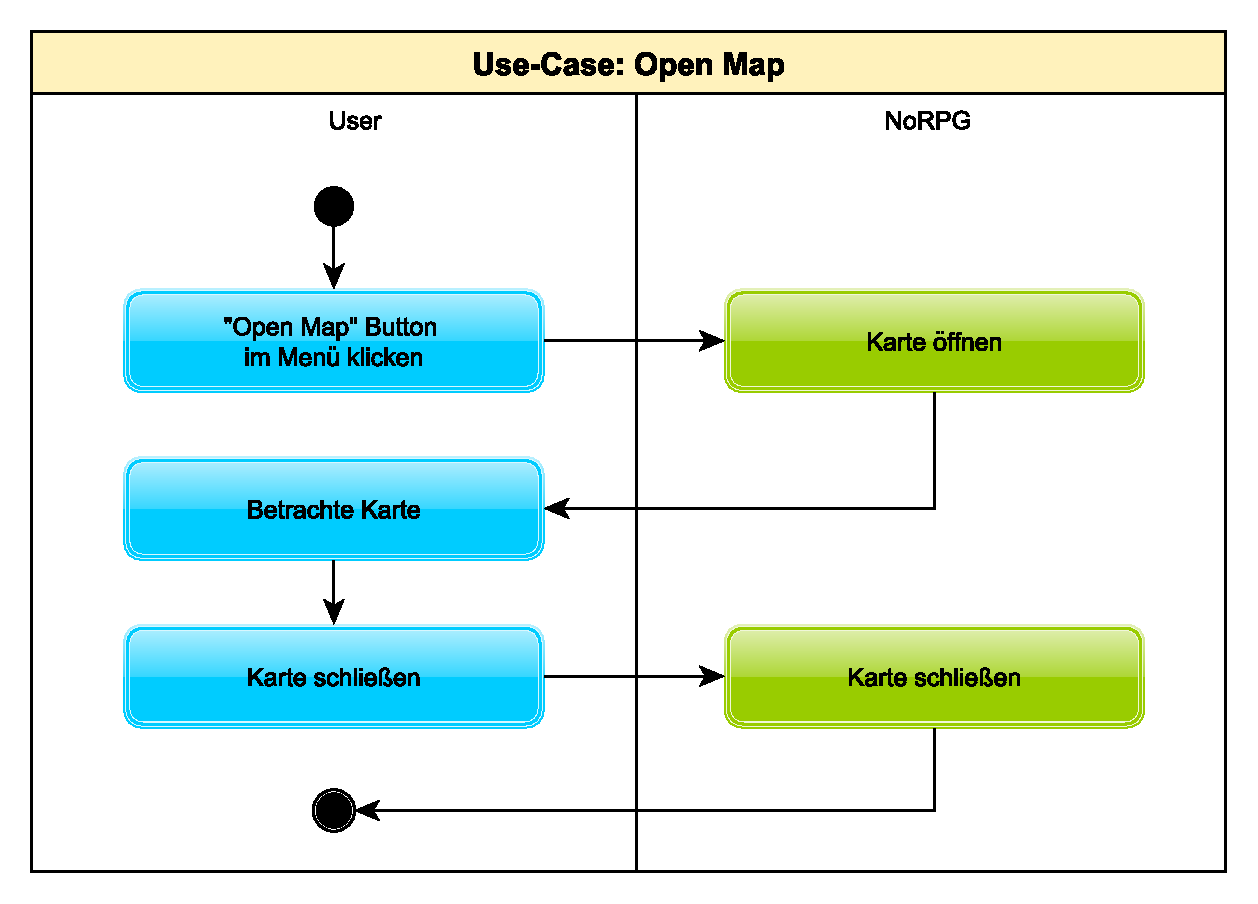
\includegraphics[width=10cm]{pics/OpenMap.pdf}
		\caption{Activity Diagramm: Open Map}
	\end{figure}

	\begin{figure}[htbp]
		\centering 
		\label{umlViewProgess}
		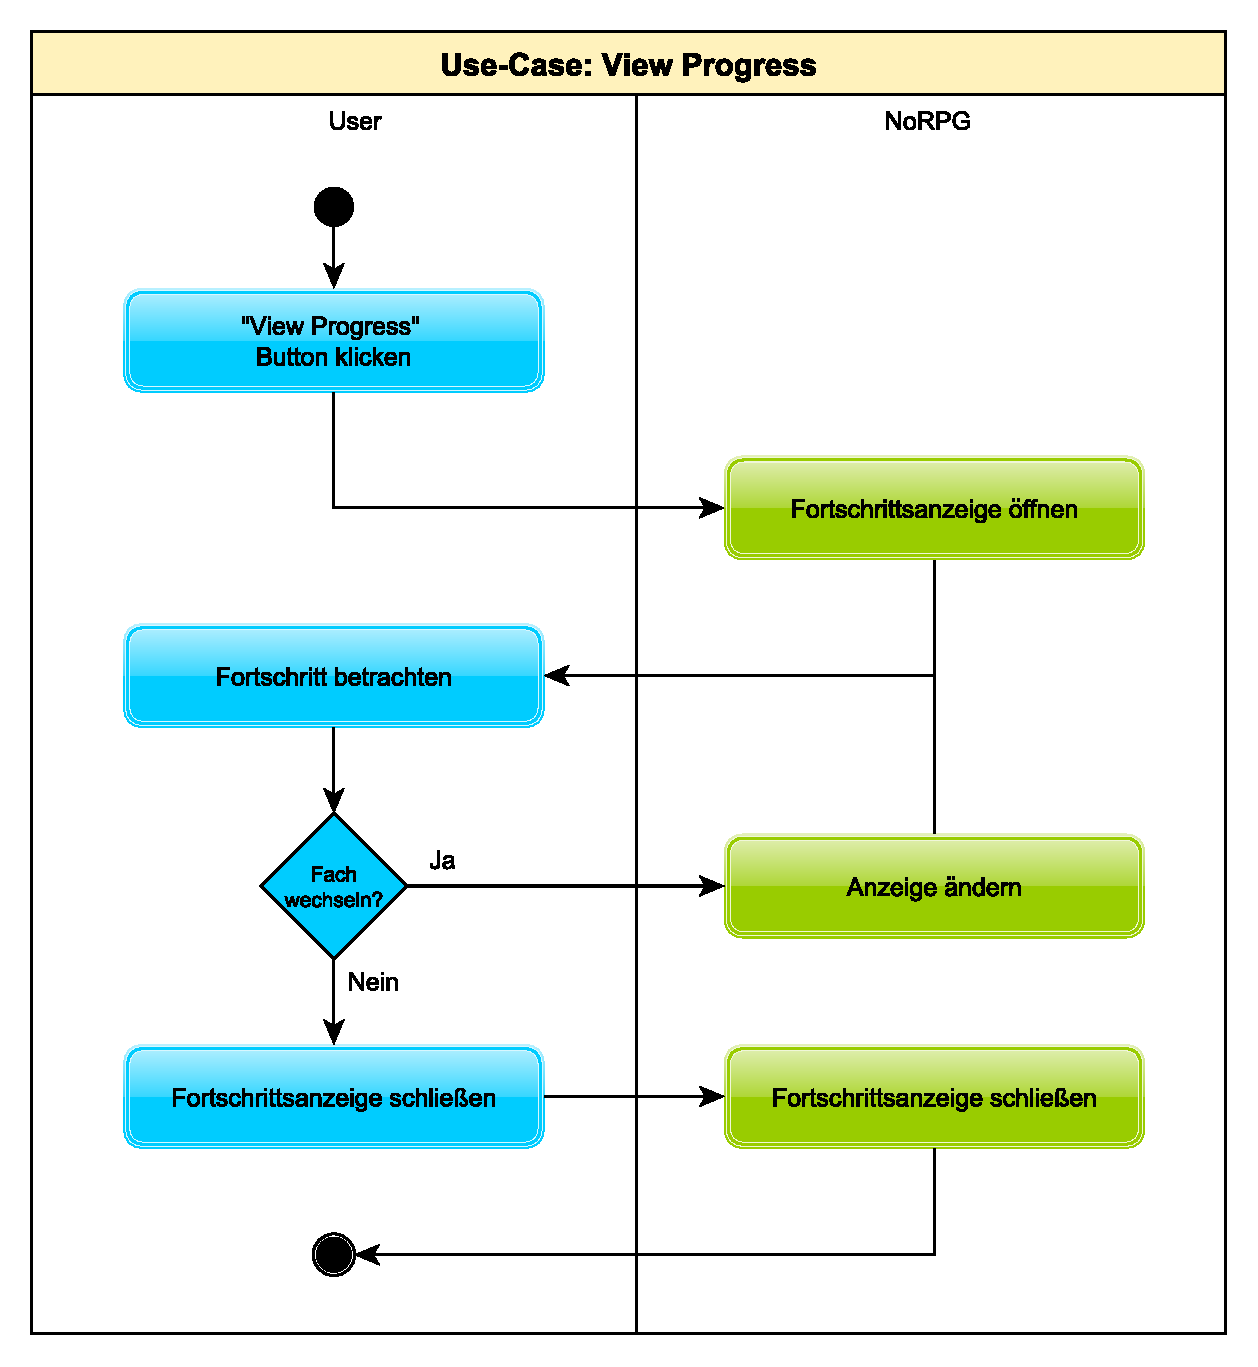
\includegraphics[width=10cm]{pics/ViewProgress.pdf}
		\caption{Activity Diagramm: View Progress}
	\end{figure}

\end{document}